%to produce a pdf, you type: pdflatex thissample
%pdflatex can imports pdf files and eps files with the \includegraphics command.  PDFs need (last time I checked) the source file whatever.pdf to be called as whatever.eps in the LaTeX file. It will then use the whatever.eps file if it exists and its creation date is more recent than whatever.pdf. If the .eps file is older or missing, it uses whatever.pdf. If it uses the .eps file, it also replaces the .pdf file with this newer image.
%Note that there is also \resizebox{<width>}{<height>}{<content>} which allows you to scale the image to a given size. This can be more useful for adjusting bigger graphics or pictures: \resizebox{\textwidth}{!}{<content>} scales the content directly to the size of the main text. The ! for the height states that it should scale with the width. See my answer to Quickest way to include graphics for more explanation about scale vs. direct width/height.

%See the graphics/x manual for the other commands like \rotatebox. Note that if you want to resize images you can use the optional arguments of \includegraphics[height=<height>,width=<width>,angle=<angle>,keepaspectratio]{<filename>}.
%usepackage microsize????????????????????
% >>>>>>>>>>>>>>>>>>>>>>   see line 214 for black and white vs black red and white <<<<<<<<<<<<<<<<<<<<<<<<<<< B^W conversion: next line
% gs -sOutputFile=000friver.pdf -sDEVICE=pdfwrite -sColorConversionStrategy=Gray -dProcessColorModel=/DeviceGray  -dCompatibilityLevel=1.4 00friver.pdf
%betterway: use adobepro select printproduction preflight click on covert to greyscale then analyze and fix button may need to go to View tab & Tools
%% and type Q no needs return %% COMPLETE with quit Turns color to stipple.
\RequirePackage{fix-cm}
%\documentclass[12pt, makeidx]{book} \usepackage[dvips]{graphics} \usepackage{graphicx} \usepackage{epsfig}
\documentclass[pdftex,12pt, makeidx]{book} \usepackage[dvips]{graphics} \usepackage{graphicx} \usepackage{epsfig}
%%%\documentclass[12pt,draft, makeidx]{book} \usepackage[dvips]{graphics} \usepackage[final]{graphicx} \usepackage{epsfig}
%%%\\documentclass[12pt,draft, makeidx]{book} \usepackage[dvips,draft]{graphics} \usepackage[draft]{graphicx} \usepackage[draft]{epsfig}
%USE COMMENT BELOW INSTEAD


\usepackage[dvips]{color}
\usepackage[T1]{fontenc} 
%\usepackage{ae,aecompl} 
%\usepackage[varg]{txfonts}
%\usepackage[px]{sfmath}
%\usepackage{pxfonts} %flaky math bold and others
\usepackage[light,condensed]{iwona} %
%\usepackage[utopia]{mathdesign}  %nice   are??? are sans??
%\usepackage{cmbright}  
%\usepackage{mathtime}
%\usepackage{mathptmx}
%\usepackage{mbtimes}
%\usepackage[charter]{mathdesign} %more readable?
%\usepackage[garamond]{mathdesign}
%\usepackage{fourier}
%\usepackage{pxfonts} 
%\usepackage{pxfonts} 
%\usepackage{times}  
\usepackage{graphicx}
\usepackage{stackrel}
\usepackage{truncate}
%\usepackage{extarrows}
\usepackage{amsmath,amssymb}
\usepackage{stmaryrd}
\usepackage[hang,small,bf,textfont=it]{caption}
\usepackage[hang]{subfigure}
\usepackage[all]{xy}
%\usepackage{url}
\usepackage{calc}
\usepackage{float}
%\usepackage[lineno5]{lgrind}
%\usepackage{alltt}
\usepackage[normalem]{ulem}
\usepackage[usenames,dvipsnames]{xcolor}
\usepackage{soul}
\usepackage{rotating}
\usepackage{anyfontsize}
\usepackage{sidecap}
\usepackage{latexsym}
%\usepackage{CJKutf8} %<<<<<<<<<<<<<<<<<<<<<<<<<<<<<<<<<<<<<<<<<CHINESE
%\AtBeginDvi{\input{zhwinfonts}}
\usepackage[scr=boondoxo,scrscaled=1.05]{mathalfa}
\usepackage{epstopdf}

\def\ZOOOO{\begin{exercise}}
\def\OOOOZ{\end{exercise}}
\definecolor{XXX}{rgb}{0,0,0}

\def\whereis{??}
\def\CH{}
\def\SECT{}
\usepackage{fancyhdr}
\def\mathbf#1{\boldsymbol{#1}}        %new def March25 2012.
\pagestyle{fancy}
\fancyhf{}
%\lhead{\footnotesize \parbox{\hsize}{Custom left-head-note} }
%\lhead{\footnotesize \parbox{11cm}{\thechapter~\CH}}
%\lfoot{\footnotesize \parbox{11cm}{\whereis}}
%\rfoot{\tiny \parbox{11cm}{{$\whereis$}}}
\setlength{\headheight}{14.5pt}
\setlength{\parindent}{1.6em}
%\renewcommand\footrulewidth{0.4pt}
\renewcommand\headwidth{\HHSIZE} 
\setlength{\headsep}{12pt}
\setlength{\voffset}{-.5in}
\setlength{\footskip}{0in}
\renewcommand{\topfraction}{0.99}	% max fraction of floats at top
    \renewcommand{\bottomfraction}{0.99}	% max fraction of floats at bottom
    %   Parameters for TEXT pages (not float pages):
    \setcounter{topnumber}{2}
    \setcounter{bottomnumber}{2}
    \setcounter{totalnumber}{4}     % 2 may work better
    %\setcounter{dbltopnumber}{2}    % for 2-column pages
    %\renewcommand{\dbltopfraction}{0.9}	% fit big float above 2-col. text
    \renewcommand{\textfraction}{0.00}	% allow minimal text w. figs
    %   Parameters for FLOAT pages (not text pages):
    \renewcommand{\floatpagefraction}{0.95}	% require fuller float pages
	% N.B.: floatpagefraction MUST be less than topfraction !!
    \renewcommand{\dblfloatpagefraction}{0.9}	% require fuller float pages

\definecolor{White}{rgb}{.0,.0,.0}

\def\caja{\mathsurround=0pt}
\def\eqalign#1{\,\vcenter{\openup1\jot \caja
        \ialign{\strut \hfil$\displaystyle{##}$&$
        \displaystyle{{}##}$\hfil\crcr#1\crcr}}\,}


\renewcommand{\baselinestretch}{.95}

%copied from web edited to remove errors puts to much space before the = sign  but runs
\newskip\humongous \humongous=0pt plus 1000pt minus 1000pt
        \ialign{\strut \hfil$\displaystyle{#}$&$
        \displaystyle{{}#}$\hfil\crcr\crcr}
\newif\ifdtup
\def\panorama{\global\dtuptrue \openup1\jot \caja
        \everycr{\noalign{\ifdtup \global\dtupfalse
        \vskip-\lineskiplimit \vskip\normallineskiplimit
        \else \penalty\interdisplaylinepenalty \fi}}}
\def\eqalignno#1{\panorama \tabskip=\humongous 
        \halign to\displaywidth{\hfil$\displaystyle{##}$
        \tabskip=0pt&$\displaystyle{{}##}$\hfil 
        \tabskip=\humongous&\llap{$##$}\tabskip=0pt
        \crcr#1\crcr}}


\usepackage{makeidx}

\setlength{\captionmargin}{20pt}
\textwidth = 42.0pc
\textheight = 56.pc      %% CHECKTHIS!!!!!!!!!!!!!!!!!!!!!!!!!!!!
\oddsidemargin = 0pc
%\evensidemargin = -3pc Done on line 205  For printed book
%\topmargin = -1.1pc
%\topmargin = 5.0pc
\topmargin = -0.3pc

\hbadness = 10000
\tolerance = 1000
\vbadness = 10000

\input{epsf}

\newlength{\contindent}
\newlength{\HHSIZE}
\newlength{\hHSIZE}
\newlength{\vZQOo}
\newlength{\vZQOe}
\newlength{\vZQOp}
\newlength{\ZQOo}
\newlength{\ZQOe}
\newlength{\ZQOp}
\def\contentsname{\vspace*{-.95in}Contents\vspace*{-.6in}}

\let\tcolor\color
\def\color#1{}
\let\tcolorbox\colorbox
%\def\colorbox#1{}

\def\SHOWfigs#1{\smash{\raise -1.8ex\hbox to0in{\hspace{-3in}#1}}}
\let\eeepsfig\epsfig
\def\epsfig#1{\eeepsfig{#1}\SHOWfigs{#1}} 
\message{COMMENTComment to show fig file names, and then RUN silently}
\message{Comment to show fig file names, and run silently}
\message{Comment to show fig file names, and run silently}
\def\SHOWfigs#1{} %<<<<<<<<<<<<<<<<<<<<<<<<<<<<<<<<<<<<<<<<<<<<<<<<<<<<<<<<<<<<<<<<<<<<<<<<<<<<<<<<<<<<<<<<<<<<<<<
\message{Comment to show fig file names, and run silently}
\message{Comment to show fig file names, and run silently}
\message{Comment to show fig file names, and run silently}

\let\eepsfig\epsfig
\def\XXXXX{}

\def\epsfbox#1{\epsfig{file={#1}}}
%		UNCOMMENT V to print figs and codes only. UNComment here
%\def\XXXXX{\newpage}\tcolor{white}\let\tcaption\caption\def\caption#1{\tcaption{\textcolor{black}{#1}}}
%		UNCOMMENT ^ to print figs and codes only.
%to print figs and progs only with all else white 


\message{UNCOMMENT THIS FOR SCROLLING    |  }
\message{UNCOMMENT THIS FOR SCROLLING    |  }
\message{UNCOMMENT THIS FOR SCROLLING    |  }
\message{UNCOMMENT THIS FOR SCROLLING    |  }
\message{UNCOMMENT THIS FOR SCROLLING    |  }
\message{UNCOMMENT THIS FOR SCROLLING    |  }
\message{UNCOMMENT THIS FOR SCROLLING  \ | /}
\message{UNCOMMENT THIS FOR SCROLLING   \|/ }
\message{UNCOMMENT THIS FOR SCROLLING    V  }    %for scrolling  UNCOMMENT  FOR
%%%%%%%%%%%%%%%%%%%%%%%%%                                   SCROLLING works as pdf NOT as ps
%\special{papersize=8.5in,9.1in} \evensidemargin=0pc \setlength{\paperheight}{9.1in}\topmargin= -1.45in
\message{UNCOMMENT THIS FOR SCROLLING    |  }    %for scrolling  UNCOMMENT  UNComment
\message{UNCOMMENT THIS FOR SCROLLING   /|\ }
\message{UNCOMMENT THIS FOR SCROLLING  / | \ }
\message{UNCOMMENT THIS FOR SCROLLING    |  }


\def\epsfig#1{\colorbox{yellow}{\eepsfig{#1}}}\let\color\tcolor\let\colorbox\tcolorbox  %leave for shading in B&W Instead, change red to black below
%		  UNCOMMENT FOR no red text       |
%		  UNCOMMENT FOR no red text       |
%		  UNCOMMENT FOR no red text.      |
%		  UNCOMMENT FOR no red text.   \  |  /
%		  UNCOMMENT FOR no red text.    \ | /
\evensidemargin = -0pc     %                     \|/
%\definecolor{red}{rgb}{0,0,0} \evensidemargin = -3pc %%%%%%%%%%%%%%%% uncomment to change red code to color to black 
%%%Unix command below turns color pdf to B&W but red is a little light. So use ^^ to turn red type to black
% gs -sOutputFile=000friver.pdf -sDEVICE=pdfwrite -sColorConversionStrategy=Gray -dProcessColorModel=/DeviceGray  -dCompatibilityLevel=1.4 00friver.pdf
%AcrobatPro has a better option: the mulitcolor button in acrobat pro
\message{UNCOMMENT THIS FOR no red           |   }         %% and type Q no needs return %% COMPLETE with quit
\message{UNCOMMENT THIS FOR no red          /|\  }
\message{UNCOMMENT THIS FOR no red         / | \ }
\message{UnCOMMENT THIS FOR no red           |   }
\message{UnCOMMENT THIS FOR no red           |   }
\message{UnCOMMENT THIS FOR no red           |   }
\message{UnCOMMENT THIS FOR no red           |   }

\makeatletter
\renewcommand{\@pnumwidth}{2.0em}% default is 1.55em  for page #s in TOC
\makeatother
\renewcommand{\topfraction}{0.85}
\renewcommand{\textfraction}{0.1}
\renewcommand{\floatpagefraction}{0.75}
\newlength{\templength}
\newlength{\templengthp}

\let\em\it
\let\sl\it
\def\emph#1{\textit{#1}\/}
\def\wavearrow{\rightarrow}
            %%%%%%%%%%%%%%%%% turns color into grayscale %%%%%%%%%%%%%%%%%%%%%%%%%%%%%%%%%%%
% gs -sOutputFile=000friver.pdf -sDEVICE=pdfwrite -sColorConversionStrategy=Gray -dProcessColorModel=/DeviceGray  -dCompatibilityLevel=1.4 00friver.pdf
% gs -sOutputFile=001friver.pdf -sDEVICE=pdfwrite -sColorConversionStrategy=Gray -dProcessColorModel=/DeviceGray  -dCompatibilityLevel=1.4 01friver.pdf
% gs -sOutputFile=002friver.pdf -sDEVICE=pdfwrite -sColorConversionStrategy=Gray -dProcessColorModel=/DeviceGray  -dCompatibilityLevel=1.4 02friver.pdf

% gs -sOutputFile=biniou.pdf -sDEVICE=pdfwrite \
%  -sColorConversionStrategy=Gray -dProcessColorModel=/DeviceGray \
%  -dCompatibilityLevel=1.4 Plot.pdf

%\setcounter{PageFW}{\thepage}
% on page \thePageFW 
%\documentstyle[11pt,twoside,yaa]{article}
%\textwidth = 42.0pc
%\textheight = 54.0pc
%\oddsidemargin = 0pc
%%\evensidemargin = -3pc
%\evensidemargin = 0pc
%\topmargin = -1.0pc
%%\newcommand{\pyind}{2em}% linenumber spacing
%\include{qrogram}
%
%\pagestyle{yaa}
%
%\begin{document}
%%\zmarkboth{Recurrence Equations}
%\zmarkright{Executive Summary}
%\zmarkcr{Siegel, 1993}
%\let\Include=\include
%\def\include#1{\zbot{#1}\Include{#1}}
\def\noop#1{}
\def\showtime#1#2#3{\par\noindent\hbox{\hbox to .45\hsize{#1}\hbox to 4em{\hfil#2\hfil}\hbox{#3}}}
\def\KKQ{{\it BigEnuf}}

\def\inset#1{{
{\par\noindent\hangafter=0\hangindent=2em
\textwidth-4em
#1}}}

\def \LaTeX{\hbox{L\hspace{-3pt}\raise1.5pt\hbox{\footnotesize A}$\!$T\hspace{-3pt}\raise-4pt\hbox{E}$\!$X}}
\font\tenrm=cmr10
\def\Hint#1{\hfill\break Hint: #1}
\def\E{{\bf\rm E}}
\def\Var{\hbox{\bf\rm var}}
\def\Re{{\mathcal{R}}}
\def \wave{{\lower 1.1ex\hbox{$\widetilde{{\hspace*{3.0ex}}}$}}}
%\def\eee{{\tt e}}

\let\INPROC=F
\let\INPROCA=F
\let\INPROCB=F
\let\INPROCC=F

\def\rmarc#1{%
\hbox to 0em{$\stackrel{\textstyle\hbox{\raise-.6ex\hbox{$\frown$}}}%
{\raise -.25ex\hbox{\phantom{#1}}}$}{#1}}

\def\MYSPACE{}
\def\NEWSPACE{$\hbox to 1in{~~~}$}

%   \binampersand  &&&&& This is defined somewhere in a library that is used.

\def\Larc#1{%
\hbox to 0em{$\stackrel{\textstyle\,\,\,\hbox{\raise-.6ex\hbox{${\Large \frown}$}}}%
{\raise -.25ex\hbox{\phantom{$#1$}}}$}{#1}}

\def\arc#1{%
\hbox to 0em{$\stackrel{\textstyle\,\,\,\hbox{\raise-.6ex\hbox{$\frown$}}}%
{\raise -.25ex\hbox{\phantom{#1}}}$}{#1}}


%\setcounter{PageFW}{\thepage}
% on page \thePageFW 
\def\larc#1{\rmarc{#1}}

\def\DVEC#1{%
\hbox to 0em{$\stackrel{\textstyle\hbox{\raise-.6ex\hbox{$\longrightarrow$}}}%
{\raise -.25ex\hbox{\phantom{$#1$}}}$}
\hbox to 0em{$\stackrel{\textstyle\hbox{\raise-.6ex\hbox{$\longleftarrow$}}}%
{\raise -.25ex\hbox{\phantom{$#1$}}}$}{#1}}

\def\LVEC#1{%
\hbox to 0em{$\stackrel{\textstyle\hbox{\raise-.6ex\hbox{$\longrightarrow$}}}%
{\raise -.25ex\hbox{\phantom{$#1$}}}$}{#1}}

\def\VEC#1{%
\hbox to 0em{$\stackrel{\textstyle\hbox{\raise-.6ex\hbox{$\rightarrow$}}}%
{\raise -.25ex\hbox{\phantom{$#1$}}}$}{#1}}

\def\wavearrow{\leadsto}
%\def\wavearrow{{\lower 1.1ex\hbox{$\widetilde{{\hspace*{3.0ex}}}$}}\!\!\!\raise.1ex\hbox{$\scriptscriptstyle>$} \,}
\def\Sinput#1{\input{solutions/#1}}
\newcommand{\sinput}[1]{\input{solutions/#1}}
\newcommand{\zection}[1]{\setcounter{section}{-1}\section{#1}}
\setlength{\parskip}{1ex}
\newlength{\RAISER}
\newlength{\kraise}
\newlength{\craise}
\newlength{\pyind}
\newlength{\Cyind}
\newlength{\pyindconst}
\newlength{\Pparskip}
\setlength{\pyindconst}{2.5em}% linenumber indentation space HERE!!!!!!!!!!!!!!!!!!!!!!!!!!!!!!!!!!!!!
\setlength{\pyind}{\pyindconst}% linenumber spacing and here!!!!!!!!!!!!!!!!!!!!!!!!!!!!!!
%\newcommand{\myind}{2em}% nesting indentation
\newcommand{\myind}{1em}% nesting indentation NEW!
\newcommand{\Tmyind}{1em}% Typenesting indentation
\newcommand{\Bf}{\bf}% key word font
\newcommand{\Com}{\it}% Comment font
\let\TT\tt  % logic font
\newcommand{\Exit}{{\TT exit }}
\newcommand{\Exitloop}{{\TT exit repeat loop}}
%\def\Or{{\TT OR }}
%\newcommand{\Not}{\,{\small\sc NOT }}
\def\Not{\,{\hbox{\small\sc not }}}
%\newcommand{\True}{{\small\sc True }}
\def\True{{\hbox{\small\sc True} }}
%\newcommand{\Truep}{{\small\sc TRUE}}
\def\Truep{{\hbox{\small\sc True}}}
\newcommand{\Bool}{{\TT Boolean}}
\newcommand{\String}{{\TT string}}
\newcommand{\Char}{{\TT character}}
\newcommand{\Integer}{{\TT integer}}
\newcommand{\Set}{{\TT set}}
\newcommand{\Real}{{\TT real}}
%\newcommand{\False}{{\small\sc False }}
\def\False{{\hbox{\small\sc False} }}
\def\Falsep{{\hbox{\small\sc False}}}
%\newcommand{\Falsep}{{\small\sc False}}
\newcommand{\Concat}{{\TT concat }}
\newcommand{\Create}{{\TT create }}
\newcommand{\Nil}{{\TT Nil}}
\newcommand{\Nota}{{\TT Nil}}
\newcommand{\Swap}{{\TT Swap}}
\newcommand{\Free}{{\TT Free}}
\newcommand{\GoTo}{{\TT GoTo }}
\newcommand{\Const}{{\TT const}}
\newcommand{\Local}{{\TT local} }
\newcommand{\LOCAL}{{\TT local} }
%$\def\Cand{{\hbox{$\mathbf{\scriptstyle AndIfsoThenif}$} }}
%\def\Cand{{\hbox{$\mathbf{\scriptstyle ShortCAnd}$} }}
%\newcommand{\Cand}{{\TT AndIfsoThenif }}
%\newcommand{\Cor}{{\TT ORelseif }}
%\def\Cor{{\hbox{$\mathbf{\scriptstyle ShortCOr}$} }}
%\def\Cor{{\hbox{$\mathbf{\scriptstyle Orelseif}$} }}
\def\Cand{\scalebox{1}[1.45]{\hbox{\textbf{\textit{\scriptsize Andthenif}}}} }
\def\Cor{\scalebox{1}[1.45]{\hbox{\textbf{\textit{\scriptsize Orelseif}}}} }
\def\And{\,\scalebox{1}[1.45]{\hbox{$\textbf{\scriptsize And}$}}\,}
\def\Or{\,\scalebox{1}[1.45]{\hbox{$\textbf{\scriptsize Or}$}}\,}
\newcommand{\Alias}{{\TT alias }}
\newcommand{\Visible}{{\TT visible }}
\newcommand{\PushOnTo}{{\TT PushOnTo}}
\newcommand{\Push}{{\TT Push }}
\newcommand{\Pop}{{\TT Pop}}
\newcommand{\Formerly}{{\TT Formerly}}
\newcommand{\Deleted}{{\tt Deleted}}
\newcommand{\Default}{{\TT Default}}
\newcommand{\RemoveFrontOf}{{\tt RemoveFrontOf}}
\newcommand{\Deletemin}{{\hbox{\Bf deletemin} }}
\newcommand{\jOin}{{\tt Join}}
\newcommand{\eee}{{\mathbf{e}}}
\newcommand{\scE}{{\textbf{E}}}
\newcommand{\CreateEmptyStack}{{\tt CreateEmptyStack}}
\newcommand{\Exercise }{{{\bf Exercise} }}
\newcommand{\New}{{\tt New}}
\global\let\BRACK=F
\newcommand{\LBRAK}{\if T\BRACK\llap{$\lbrace$ }\global\let\BRACK =F\fi}

\setlength{\kraise}{0pt}
\setlength{\craise}{0pt}
\def\ttree{2\hspace{0pt}\raise 1pt\hbox{\small -}\hspace{-1.1pt}3\hspace{.4pt}{{\normalsize t}}ree}
\def\Ttree{2\raise.2ex\hbox{\scalebox{.6}[1]{-}}\hspace{-.2ex}3\scalebox{1}[1.3]{t}ree}
\def\TtreE{2\hspace{0pt}\raise 1.5pt\hbox{\small -}\hspace{-1.1pt}3\hspace{.4pt}{{\large t}}ree}
\def\Tsubtree{2\raise.2ex\hbox{\scalebox{.6}[1]{-}}\hspace{-.2ex}3sub\scalebox{1}[1.3]{t}ree}
%\def\Tsubtree{2\hspace{0pt}\raise 1.5pt\hbox{\small -}\hspace{-1.1pt}3\hspace{.4pt}subtree}
%\def\TTREE{{2}\hspace{0pt}\raise .35ex\hbox{\small -}\hspace{-1.1pt}{3}\hspace{.4pt}{{\huge t}}ree}%global\let\TTREE\ttree}
\def\bigt{{\fontsize{15}{17}\selectfont t}}
\def\BIGT{{\fontsize{20}{25}\selectfont t}}
\def\ums{{\uppercase{ums}}}
\def\asics{{\uppercase{asics}}}
\def\rrors{{\uppercase{rrors}}}
\def\heta{{\uppercase{heta-Oh}}}
\def\olys{{\uppercase{$\!$olynomials versus exponentials}}}
\def\olynomials{{\uppercase{$\!\!$olynomials versus exponentials}}}
%\def\TTREE{{2}\hspace{0pt}\raise-.3ex\hbox{\raise .5ex\hbox{\small -}}\hspace{-1.1pt}{3}\hspace{.4pt}\BIGT{}ree}
\def\TTREE{{2}\hspace{0pt}\raise\craise\hbox{\raise-2pt\hbox{\raise .8ex\hbox{\small -}}}\hspace{-1.1pt}{3}\hspace{.4pt}\BIGT{}ree}
%\def\TTREE{{2}\hspace{0pt}\raise .35ex\hbox{\small -}\hspace{-1.1pt}{3}\hspace{.4pt}\BIGT{}ree}
\def\rminus{\raise .29ex\hbox{{\small -}}}
%\def\RMINUS{\raise .45ex\hbox{{\small -}}}
%\def\RMINUS{\raise 3pt\hbox{{\small -}}}
\def\RMINUS{\raise\kraise\hbox{\raise 1.35ex\hbox{\raise -6pt\hbox{{\small -}}}}}
\def\Btree{B\hspace{-.9pt}\rminus\hspace{-.9pt}tree}
\def\BTREE{B\hspace{-1.1pt}\RMINUS\hspace{-.8pt}tree}

%\newlength{\MMsize}   %UPSIDE DOWN HINT PRINTER
\newlength{\Lapsize}
\newlength{\MTsize}
\newlength{\MMTsize}
%\setlength{\MMsize}{\hsize}
\setlength{\MMTsize}{\widthof{{\bf Hint}:~~}}
%\addtolength{\MMsize}{-\MMTsize} %I do not understand what \MMsize is.

\def\tniHH#1{%
\par
\noindent
{\bf Hint}:~~\reflectbox{\parbox{\hsize-\MMTsize}{#1}}}

\def\HHint#1{%
\par
\setlength{\MTsize}{\widthof{#1}}%
\addtolength{\MTsize}{\MMTsize}
\ifdim\MTsize<\hsize\par\noindent{\bf Hint}{:~}\rotatebox{180}{\raise-1ex\hbox{#1}}\else%
\par\noindent{{\bf Hint}:~~}\rotatebox{180}{\parbox{\hsize-\MMTsize}{#1}}\fi\break}

\def\KKint#1{%
\par
\setlength{\MTsize}{\widthof{#1}}%
\addtolength{\MTsize}{\MMTsize}
\ifdim\MTsize<\hsize\par\noindent{\bf Hint}{:~}\rotatebox{180}{\raise-1ex\hbox{#1}}\else%
\addtolength{\MMTsize}{4em}\par\noindent{$\hbox to4em{}${\bf Hint}:~~}\rotatebox{180}{\parbox{\hsize-\MMTsize}{#1}}\addtolength{\MMTsize}{-4em}\fi\break}

\def\Ans#1#2{%
\setlength{\MTsize}{\widthof{#1}}%
\setlength{\MMTsize}{\hsize}%
\addtolength{\MMTsize}{-\MTsize} 
\addtolength{\MMTsize}{-1ex} 
\par\noindent#1~{\rotatebox{180}{\raise-1ex\hbox{\parbox{\MMTsize}{#2}}}}}
%\ifdim \MTsize<\MMsize\ccitem{#1:~}\rotatebox{180}{\raise-1ex\hbox{#2}}\else%
%\ccitem{#1:~}\rotatebox{180}{\parbox{\MMsize}{#2}}\fi}
\def\AAns#1#2{%
\setlength{\MTsize}{\widthof{#1}}%
\setlength{\MMTsize}{\hsize}%
\addtolength{\MMTsize}{-\MTsize} 
\addtolength{\MMTsize}{-3.5ex} 
\par\noindent#1~{\rotatebox{0}{\hbox{\parbox{\MMTsize}{#2}}}}}

%\def\mod{\tt\,\,\, mod\,\,}
\def\mod#1{~(\,{\tt mod}\,#1\,)}
\newcommand{\Mod}{\tt mod\,\,}

\newcommand{\Global}{{\tt global }}
\newcommand{\GLOBAL}{{\tt global }}
\newcommand{\Ghost}{\hphantom{\tt global }}

%\newcommand{\Global}{{\Zippar\tt Global }}
%\newlength{\Zypp}
%\def\Zippar{\setlength{\Zypp}{\pyind}\addtolength{\Zypp}{\tabby}\addtolength{\Zypp}{2em}\noindent\hangafter=1\hangindent=\Zypp}
%\def\Zipout{\hangindent=0pt}
\def\Definition{\vskip .1in\noindent\hangafter=1\hangindent=2em\hbox{\Bf Definition}}
%\def\problem{Problem.}
\def\prob#1{prob\{#1\}}
\def\Defn#1{\par\penalty-500\vskip 10pt\noindent{\bf Definition\if-#1.\else
  { #1.}\fi}} %\smallskip
\def\DDefn#1{\par\penalty-500\vskip 10pt\noindent\hangafter=1\hangindent=2em{\bf Definition\if-#1.\else
  { #1.}\fi}} %\smallskip
\def\COR#1{\par\penalty-500\vskip 10pt\noindent{\bf Corollary\if-#1.\else
  { #1.}\fi}} %\smallskip
\def\Thm#1{\par\penalty-500\vskip 10pt\noindent{\bf Theorem\if-#1.\else
  { #1.}\fi}} %\smallskip
\def\Lemma#1{\par\penalty-500\vskip 10pt\noindent{\bf Lemma\if-#1.\else
  { #1.}\fi}} %\smallskip
\def\Proof{\par\noindent{\bf Proof:}\quad}

\def\blackslug{\hbox{\hskip 1pt \vrule width 4pt height 8pt depth 1.5pt\hskip
1pt}}
\def\QED{\quad\blackslug\lower 8.5pt\null}
\def\QeD{\blackslug\lower 8.5pt\null}

\def\starstar{\raise.55ex\hbox to 0in{$\star$}\raise-.55ex\hbox{$\star$}}
\def\outhang#1{\par\noindent\hangafter=1\hangindent=2em #1}

\newcommand{\evenup}{\ifodd\count0\vfill\eject\message{PAGE PADDED}
\thispagestyle{empty}
$~$\fi}
\def\oddup{\ifodd\count0\else\vfill\eject\message{PAGE PADDED}
\thispagestyle{empty}
$~$\fi}
%\def\bibitem#1{\vskip .1in\noindent\hangafter=1\hangindent=4em\hbox to 4em{#1\hfil}} %TEMP DOne in qrogram
\def\fibitem#1{\vskip .1in\noindent\hangafter=1\hangindent=4em\hbox to 4em{#1\hfil}}
\def\fibitem#1{\vskip .1in\noindent\hangafter=1\hangindent=4em\hbox to 4em{#1\hfil}}
\def\litem#1{\par\noindent\hangafter=0\hangindent=2em\hskip-2em{\bf #1}}
\def\Qitem{\par\noindent\hangafter=0\hangindent=4em\hskip-2em}
\def\citem#1{\par\noindent\hangafter=1\hangindent=2em\hbox to 2em{\hfil#1\ }}
\def\Titem#1{\par\noindent\hangafter=1\hangindent=3em\hbox to 3em{{\bf\hfil#1\ }}}
\def\Xitem#1{\par\noindent\hangafter=1\hangindent=2em\hbox to 2em{\hfil#1\ }}
\def\Yitem#1{\par\noindent\hangafter=0\hangindent=3em\llap{\hbox to 3em{\hfil#1\ }}}
\def\ccitem#1{\par\noindent\hangafter=1\hangindent=4em\hbox to 4em{\hfil#1\ }}
\def\Mitem#1{\par\noindent\hangafter=1\hangindent=2em#1}
\def\CCitem#1{\par\noindent\hangafter=1\hangindent=4em\hbox to 4em{\hfil#1}}
\def\tempdent{\par\noindent\hangafter=1\hangindent=2em}
\def\Citem#1{\par\noindent\hangafter=1\hangindent=4em\hbox to 2em{\hfil#1}}
\def\Rap{\par\noindent\hangafter=1\hangindent=1.6em}
\def\Wrap#1{\par\noindent\hangafter=1\hangindent=4ex\hbox to 2.5ex{\hfil#1~~}}
\def\WWrap#1{\par\noindent\hangafter=1\hangindent=7ex\hbox to 4ex{\hfil#1~~}}
\def\RRap{\par\noindent\hangafter=0\hangindent=3.2em}
\def\Zitem#1{\par\noindent\hangafter=1\hangindent=3.4em\hbox to 1.7em{\hfil#1}}
\def\ZZitem{\par\noindent\hangafter=0\hangindent=3.4em}
\def\KCitem#1#2{\hbox to .5\hsize{\hbox to 2em{\hfil#1}#2\hfil}}
\def\CDitem#1{\par\noindent\hangafter=1\hangindent=4em\hbox to 2em{\hfil#1}\hspace{2em}}
\def\CZitem#1{\par\noindent\hangafter=1\hangindent=5.6em\hbox to 3.6em{\hfil#1}}
\def\Qitem#1{\vspace{-2ex}\par\vspace{-1.3ex}\hangafter=1\hangindent=4em\hbox to 2em{#1}}
\def\Ditem#1#2{\noindent\parbox{\hsize-2em}{\noindent\hangafter=1\hangindent=4em\hbox to 2em{\hfil#1}#2}}
\def\Eitem{\par\noindent\hangafter=1\hangindent=2em}
\def\inditem{\par\noindent\hangafter=0\hangindent=2em}
\def\excitem#1{\par\hangafter=1\hangindent=4em{#1\ }}
\def\INDITEM{\par\hangafter=1\hangindent=4em}
\def\Excitem#1{\par\hangafter=1\hangindent=2.5em{\noindent#1\ }}
\def\Sitem#{\par\hangafter=1\hangindent=2.5em}
\def\Btem{\par\noindent\hangafter=1\hangindent=1em\hbox to1em{\hfil$\bullet$\hfil}}
\def\BBtem{\par\noindent\hangafter=1\hangindent=3em\hbox to3em{\hbox to1em{$~$}\hfil{\scriptsize$\bullet\bullet$}\hfil}}
%\def\BBtem{\par\noindent\hangafter=1\hangindent=2em\hbox to2em{\hbox to1em{$~$}\hfil{\footnotesize$\bullet$}\hfil}}
\def\dcitem#1{\par\noindent\hangafter=1\hangindent=4.2em\hbox to 4.2em{\hfil#1\ }}
\def\Dcitem#1{\par\noindent\hangafter=1\hangindent=4.5em\hbox to 4.5em{\hfil#1\ }}
\def\bitem#1{\par\noindent\hangafter=1\hangindent=4em\hbox to4em{\hfil#1\ }}
\def\BBitem#1{\par\noindent\hangafter=1\hangindent=.7em\hbox to.7em{\hfil#1\ }}
\def\Bitem#1{\par\noindent\hangafter=1\hangindent=5.5em\hbox to5.5em{\hfil#1\ }}
\def\bcitem#1{\par\noindent\hangafter=1\hangindent=6em\hbox to6em{\hfil#1\ }}
\def\PBitem#1{\par\noindent\hangafter=1\hangindent=5.5em\hbox to5.5em{\hfil\smash{\parbox[t]{5.5em}{#1}\ }}}
\def\bbitem#1{\par\noindent\hangafter=1\hangindent=8em\hbox to8em{\hfil#1\ }}
\def\bbbitem#1{\par\noindent\hangafter=1\hangindent=12em\hbox to12em{\hfil#1\ }}
\def\bbbbitem#1{\par\noindent\hangafter=1\hangindent=16em\hbox to16em{\hfil#1\ }}
\def\bitem#1{\par\noindent\hangafter=1\hangindent=4em\hbox to 4em{\hfil#1\ }}
\def\xitem#1{\par\noindent\hangafter=1\hangindent=4em\hbox to 2em{\hfil#1\ }}
\def\ceitem{\par\noindent\hangafter=1\hangindent=4em}
\def\Ceitem#1{\par\noindent\hangafter=1\hangindent=3.4em\hbox to 3.4em{#1\hfil}}
\def\Lapitem#1{\par\noindent\hangafter=1\setlength{\Lapsize}{\widthof{#1}}\hangindent=\Lapsize#1}
\def\newPr#1{\par\setlength{\xAAA}{\widthof{#1}}\addtolength{\xAAA}{0ex}\par\noindent\hangafter=1\hangindent=\xAAA#1}
%%%%\def\Cibitem{\hangafter=1\hangindent=\tabby}
\def\Moitem#1{%
\hbox to 1em{\hfil#1\ }}%
\def\moitem#1{\vspace{\parskip}\\%
\hbox to 1em{\hfil#1\ }}%
%\addtolength{\hangindent}{2em}} FLAWED
\def\parr{\par\hangafter=1\hangindent=4.2em}
\def\textvisiblespace{\texttt{\char32}}
\def\rand{\mathcal{R}{\hspace{-1pt}\it and}}
%\def\rand{{\it rand}}

\def\ProbD#1{\par\hangindent=\templengthp\hangafter=1\noindent\hbox to \templength{\underline{Definition}}:~{\bf #1}.}
\def\Question{\par\vspace{-1ex}\par\hangindent=\templengthp\hangafter=1\noindent\hbox to\templength{\hfil\underline{Question}}:~}
\def\Instance{\par\vspace{-1ex}\par\hangindent=\templengthp\hangafter=1\noindent\hbox to\templength{\hfil\underline{Instance}}:~}
\newcommand{\Problem}[1]{\par{\bf Problem}#1\par}

%\let\thefootnote\relax\footnote
%\renewcommand{\thefootnote}{\fnsymbol{footnote}}
%\def\Fnote#1#2{{\footnote{}{{\zoo\tenrm\baselineskip 16pt
%\vskip -1em\par\noindent\hangafter=1\hangindent=20truept
%\hbo

%\def\Footnote#1#2{{${}^{\rm #1}$\Fnote{#1}{#2}}}
\def\Footnote#1{\footnote{#1}}

\global\let\NORMALIF = A
\global\let\COMMY = N

%\newcommand{\Newline}{\newline}
%\newcommand{\Newline}{\if T\newl{\\}\else{\global\let\newl = T}\fi}
\newcommand{\Newline}{\if T\newl\hfil\break\else\global\let\newl = T\fi}

\newcommand{\MprogA}{%
\global\setcounter{linenumbA}{\thelinenumb}%
\global\let\INPROCA=\INPROC%
\global\setlength{\tabbyA}{\tabby}%
\global\setlength{\ClengthA}{\CClength}}

\newcommand{\MprogB}{%
\global\setcounter{linenumbB}{\thelinenumb}%
\global\let\INPROCB=\INPROC%
\global\setlength{\tabbyB}{\tabby}%
\global\setlength{\ClengthB}{\CClength}}

\newcommand{\MprogC}{%
\global\setcounter{linenumbC}{\thelinenumb}%
\global\setlength{\tabbyC}{\tabby}%
\global\let\INPROCC=\INPROC%
\global\setlength{\ClengthC}{\CClength}}

\newcommand{\MprogD}{%
\global\setcounter{linenumbD}{\thelinenumb}%
\global\let\INPROCD=\INPROC%
\global\setlength{\tabbyD}{\tabby}%
\global\setlength{\ClengthD}{\CClength}}

\newcommand{\MprogE}{%
\global\setcounter{linenumbE}{\thelinenumb}%
\global\let\INPROCE=\INPROC%
\global\setlength{\tabbyE}{\tabby}%
\global\setlength{\ClengthE}{\CClength}}

\newcommand{\declnumb}[1]{\addtocounter{lilinenumb}{-1}}
\newcommand{\Llnumb}[1]{\setcounter{lilinenumb}{#1}}
\newcommand{\Lnumb}[1]{\setcounter{linenumb}{#1}}

\def\Pr#1{\hbox{Pr}\{#1\}}
\newcommand{\ProgA}{\global\def\Fini{\normalcolor}%
\color{red}\setcounter{linenumb}{\thelinenumbA}\global\let\newl=F
\setlength{\pyind}{\pyindconst}% linenumber spacing
%\addtocounter{linenumb}{-1}%new in format  Will mess some old idiot stuff
\global\let\INPROC=\INPROCA%
\setlength{\tabby}{\tabbyA}
\setcounter{lilinenumb}{0}%
\setlength{\CClength}{\ClengthA}% moved: formerly outside 
%\global\let\NORMALIF = N
\global\let\COMMY = N
\global\let\INLINE = T\par\noindent}
%\if 0\thelinenumb{\hbox to \pyind{\hfill}\hspace*{\tabby}%
%}\else{\hbox to \pyind{\hfill\thelinenumb\hbox to 1.5em{\hfil}}\hspace*{\tabby}}\fi}%begins line properly

\newcommand{\ProgAA}{\global\def\Fini{\normalcolor}%
\color{red}\setcounter{linenumb}{\thelinenumbA}\global\let\newl=F
\setlength{\pyind}{\pyindconst}% linenumber spacing
\addtocounter{linenumb}{-1}%new in format  Will mess some old idiot stuff
\global\let\INPROC=\INPROCA%
\setlength{\tabby}{\tabbyA}
\setcounter{lilinenumb}{0}%
\setlength{\CClength}{\ClengthA}% moved: formerly outside 
%\global\let\NORMALIF = N
\global\let\COMMY = N
\global\let\INLINE = T\par\noindent}
%\if 0\thelinenumb{\hbox to \pyind{\hfill}\hspace*{\tabby}%
%}\else{\hbox to \pyind{\hfill\thelinenumb\hbox to 1.5em{\hfil}}\hspace*{\tabby}}\fi}%begins line properly

\newcommand{\ProgB}{\global\def\Fini{\normalcolor}%
\color{red}\setcounter{linenumb}{\thelinenumbB}\global\let\newl=F
\setlength{\pyind}{\pyindconst}% linenumber spacing
%\addtocounter{linenumb}{-1}%new in format  Will mess some old idiot stuff
\global\let\INPROC=\INPROCB%
\setcounter{lilinenumb}{0}%
\setlength{\tabby}{\tabbyB}
\setlength{\CClength}{\ClengthB}% moved: formerly outside 
%\global\let\NORMALIF = N
\global\let\COMMY = N
\global\let\INLINE = T\par\noindent}
%\if 0\thelinenumb{\hbox to \pyind{\hfill}\hspace*{\tabby}%
%}\else{\hbox to \pyind{\hfill\thelinenumb\hbox to 1.5em{\hfil}}\hspace*{\tabby}}\fi}%begins line properly
%\hbox to \pyind{\hfill\thelinenumb\hbox to 1.5em{\hfil}}\hspace*{\tabby}}

\newcommand{\ProgC}{\global\def\Fini{\normalcolor}%
\color{red}\setcounter{linenumb}{\thelinenumbC}\global\let\newl=F
\setlength{\pyind}{\pyindconst}% linenumber spacing
%\addtocounter{linenumb}{-1}%new in format  Will mess some old idiot stuff
\global\let\INPROC=\INPROCC%
\setcounter{lilinenumb}{0}%
\setlength{\tabby}{\tabbyC}
\setlength{\CClength}{\ClengthC}% moved: formerly outside 
%\global\let\NORMALIF = N
\global\let\COMMY = N
\global\let\INLINE = T\par\noindent}
%\if 0\thelinenumb{\hbox to \pyind{\hfill}\hspace*{\tabby}%
%}\else{\hbox to \pyind{\hfill\thelinenumb\hbox to 1.5em{\hfil}}\hspace*{\tabby}}\fi}%begins line properly
%\hbox to \pyind{\hfill\thelinenumb\ \ }\hspace*{\tabby}}

\newcommand{\ProgD}{%
\color{red}\setcounter{linenumb}{\thelinenumbD}\global\let\newl=F
\setlength{\pyind}{\pyindconst}% linenumber spacing
%\addtocounter{linenumb}{-1}%new in format  Will mess some old idiot stuff
\global\let\INPROC=\INPROCD%
\setcounter{lilinenumb}{0}%
\setlength{\tabby}{\tabbyD}
\setlength{\CClength}{\ClengthD}% moved: formerly outside 
%\global\let\NORMALIF = N
\global\let\COMMY = N
\global\let\INLINE = T\par\noindent}
%\if 0\thelinenumb{\hbox to \pyind{\hfill}\hspace*{\tabby}%
%}\else{\hbox to \pyind{\hfill\thelinenumb\hbox to 1.5em{\hfil}}\hspace*{\tabby}}\fi}%begins line properly
%\hbox to \pyind{\hfill\thelinenumb\ \ }\hspace*{\tabby}}

\newcommand{\ProgE}{\global\def\Fini{\normalcolor}%
\color{red}\setcounter{linenumb}{\thelinenumbE}\global\let\newl=F
\setlength{\pyind}{\pyindconst}% linenumber spacing
%\addtocounter{linenumb}{-1}%new in format  Will mess some old idiot stuff
\global\let\INPROC=\INPROCE%
\setcounter{lilinenumb}{0}%
\setlength{\tabby}{\tabbyE}
\setlength{\CClength}{\ClengthE}% moved: formerly outside 
%\global\let\NORMALIF = N
\global\let\COMMY = N
\global\let\INLINE = T\par\noindent}
%\if 0\thelinenumb{\hbox to \pyind{\hfill}\hspace*{\tabby}%
%}\else{\hbox to \pyind{\hfill\thelinenumb\hbox to 1.5em{\hfil}}\hspace*{\tabby}}\fi}%begins line properly
%\hbox to \pyind{\hfill\thelinenumb\ \ }\hspace*{\tabby}}

\newlength{\gappy}
\newlength{\tabby}
\newlength{\tabbyA}
\newlength{\tabbyB}
\newlength{\tabbyC}
\newlength{\tabbyD}
\newlength{\tabbyE}

\def\parencheck{\ifdim \tabby=0em{}\else%
\message{WARNING: POSSIBLE Indentation mismatch}%
\message{WARNING: POSSIBLE Indentation mismatch}%
\message{WARNING: POSSIBLE Indentation mismatch}%
\message{WARNING: POSSIBLE Indentation mismatch}%
\message{WARNING: POSSIBLE Indentation mismatch}%
\message{WARNING: POSSIBLE Indentation mismatch}\fi}

\newlength{\Cind}
\setlength{\Cind}{1em}

\newlength{\cabby}
\newlength{\Offset}
\setlength{\Offset}{0in}
\newlength{\Plen}

\newlength{\Clength}
\newlength{\Plength}
\setlength{\Clength}{\textwidth}
\addtolength{\Clength}{-\pyind}
\addtolength{\Clength}{-\Cind}
\addtolength{\Clength}{-.4em}
\newlength{\zeroem}
\setlength{\zeroem}{0em}
\newlength{\CClength}
\newlength{\ClengthA}
\newlength{\ClengthB}
\newlength{\ClengthC}
\newlength{\ClengthD}
\newlength{\ClengthE}
\newlength{\xAAA}
\newlength{\xBBB}
\newlength{\xCCC}
\newlength{\xDDD}
\newlength{\xEEE}
\newlength{\xFFF}
\newlength{\xGGG}
\newlength{\xHHH}
\def\lboxed#1{\setlength{\xAAA}{\widthof{#1}}}
\def\llboxed#1{\hbox to\xAAA{#1}}
\def\rboxed#1{\setlength{\xBBB}{\widthof{#1}}}
\def\rrboxed#1{\hbox to\xBBB{#1}}
\def\Angstrom{\r{A}}
\def\AA{\r{A}}
\def\aa{\r{a}}

\def\Rightshift#1{{\noindent\vspace{0em}\noindent\hangafter=0\hangindent=\cabby}#1\vspace{0em}\noindent}

\newcounter{PageFW}
\newcounter{linenumb}
\newcounter{linenumbA}
\newcounter{linenumbB}
\newcounter{linenumbC}
\newcounter{linenumbD}
\newcounter{linenumbE}
\newcounter{lilinenumb}
\newcounter{AAA}
\newcounter{BBB}

\newlength{\Distance}

\newcommand{\Dist}{\setlength{\Distance}{\tabby}}

\newcommand{\Simulate}[1]{\hbox to
\pyind{\hfill\#1\hbox to 1.5em{\hfil}}\hspace*{\tabby}}

\newcommand{\Saveas}[2]{%
\newcounter{#1}\setcounter{#1}{#2}}
\newcommand{\Recordas}[2]{\global\def#1{#2}}
%\newcommand{\Saveas}[2]{\refstepcounter{#2}\label{#1}}

\newcommand{\Save}[1]{\newcounter{#1}\setcounter{#1}{\thelinenumb}}
%\newcommand{\Save}[1]{Saveas{#1}{\thelinenumb}}

\global\let\indented=F

\newcommand{\Progqbel}[1]{\Prog\qbel{#1}\hspace*{-\myind}\global\let\indented=T}
\newcommand{\Progpbel}[1]{\Prog\pbel{#1}\hspace*{-\myind}\global\let\indented=T}

\def\Proog{\global\def\Fini{\normalcolor}\color{red}}

\def\xPage{}
\newcommand{\Prog}{\xPage\global\def\Fini{\normalcolor}%
\color{red}\setcounter{linenumb}{0}
\setlength{\pyind}{\pyindconst}% linenumber spacing
\setlength{\tabby}{\zeroem}
\setlength{\CClength}{\Clength}% moved: formerly outside 
\global\let\newl = F%
\global\let\INPROC=F%
\global\let\indented = F
%\global\let\NORMALIF = N
\global\let\COMMY = N
\global\let\INLINE = T\par\noindent}% fixed: formerly F

\newcommand{\ProgN}[1]{\xPage\global\def\Fini{\normalcolor}%
\color{red}\setcounter{linenumb}{#1}
\addtocounter{linenumb}{-1}
\setlength{\pyind}{\pyindconst}% linenumber spacing
\setlength{\tabby}{0em}
\setlength{\CClength}{\Clength}% moved: formerly outside 
\global\let\newl = F%
\global\let\INPROC=F%
\global\let\indented = F
%\global\let\NORMALIF = N
\global\let\COMMY = N
\global\let\INLINE = T\par\noindent}% fixed: formerly F

\newcommand{\nProg}{\xPage\global\def\Fini{\normalcolor}% DOES NOT RESET LINE COUNTER
\color{red}%\setcounter{linenumb}{0}
\setlength{\pyind}{\pyindconst}% linenumber spacing
\setlength{\tabby}{0em}
\setlength{\CClength}{\Clength}% moved: formerly outside 
\global\let\newl = F%
\global\let\INPROC=F%
\global\let\indented = F
%\global\let\NORMALIF = N
\global\let\COMMY = N
\global\let\INLINE = T\par\noindent}% fixed: formerly F

\newcommand{\Rrog}{\xPage\global\def\Fini{\normalcolor}%
\color{red}\setcounter{linenumb}{0}
\setlength{\pyind}{\pyindconst}% linenumber spacing
\setlength{\tabby}{0em}
\setlength{\CClength}{\Clength}% moved: formerly outside 
\global\let\newl = F%
\global\let\INPROC=F%
\global\let\indented = F
%\global\let\NORMALIF = N
\global\let\COMMY = N
\global\let\INLINE = T}% fixed: formerly F

%\newcommand{\Prog}[1]{\setcounter{linenumb}{0}
%\setlength{\pyind}{\pyindconst}% linenumber spacing
%\setlength{\tabby}{0em}
%\setlength{\CClength}{\Clength}% moved: formerly outside 
%\if \qq#1{\global\let\newl = T}\else{\if \p#1{\global\let\newl = T}%
%\else{\global\let\newl = F}\fi}\fi%
%\global\let\indented = F
%%\global\let\NORMALIF = N
%\global\let\COMMY = N
%{\global\let\INLINE = T}\par\noindent#1}% fixed: formerly F

\newcommand{\Gorp}{\global\let\NORMALIF=A}

\newcommand{\Progq}{\global\def\Fini{\normalcolor}%
\color{red}\setcounter{linenumb}{0}\global\let\newl=T%
\setlength{\pyind}{\pyindconst}% linenumber spacing
\setlength{\tabby}{0em}
\setlength{\CClength}{\Clength}% moved: formerly outside 
\global\let\indented = T
%\global\let\NORMALIF = N
\global\let\COMMY = N
\global\let\INLINE = T
\par\noindent
\hbox to \pyind{\hfill}\hspace*{\tabby}}

\newcommand{\Progp}{\global\def\Fini{\normalcolor}%
\color{red}\setcounter{linenumb}{0}\global\let\newl=F
\setlength{\pyind}{\pyindconst}% linenumber spacing
\setlength{\tabby}{0em}
\setlength{\CClength}{\Clength}% moved: formerly outside 
\global\let\indented = T
%\global\let\NORMALIF = N
\global\let\COMMY = N
\global\let\INLINE = T
\addtocounter{linenumb}{1}
\par\noindent
\hbox to \pyind{\hfill\thelinenumb\hbox to 1.5em{\hfil}}\hspace*{\tabby}}


\newcommand{\q}{\if C\COMMY{$\rbrace$\global \let\COMMY = N}\fi\Newline%
\global\let\newl = T
\global\let\indented = T
\global\let\INLINE = T
\global\let\NORMALIF = N}

\def\qlabel#1{\if F\INPROC\global\let\indented = T\fi%%
\if C\COMMY{$\rbrace$\global \let\COMMY = N}\fi%
\global\let\INLINE = T%
\global\let\NORMALIF = N%
\global\let \NORMALREC=N%
\Newline\global\let\newl=T% the newline starts next line command
{\hbox to \pyind{\hfill#1}\hspace*{\tabby}}}


\newcommand{\qbel}[1]{\if C\COMMY$\rbrace$\global \let\COMMY = N\fi
\global\let\INLINE = T
\global\let\NORMALIF = N
\Newline % the newline starts next line command
\addtocounter{linenumb}{1}
\hbox to 1em{#1\hfill}\hspace*{\tabby}}


\newcommand{\pbel}[1]{\if C\COMMY{$\rbrace$\global \let\COMMY = N}\fi
\global\let\INLINE = T
\global\let\NORMALIF = N
\Newline % the newline starts next line command
\addtocounter{linenumb}{1}
\hbox to \pyind{\hfill\thelinenumb\hbox to 1.5em{\hfil}}\rlap{\hskip -.5em#1}\hspace*{\tabby}}


\newcommand{\plabel}[1]{\if C\COMMY$\rbrace$\global \let\COMMY = N\fi
\global\let\INLINE = T
\global\let\NORMALIF = N
\Newline % the newline starts next line command
\addtocounter{linenumb}{1}
\hbox to \pyind{\hfill\thelinenumb\hbox to 1.5em{\hfil}}\rlap{\hskip -.5em#1:}\hspace*{\tabby}}


\newcommand{\C}{\qq\global\let\INLINE=F}
%%%%\newcommand{\C}{\setlength{\Pparskip}{\parskip}\setlength{parskip}{0em}%
%%%%\global\let\INLINE=F%
%%%%\if F\INPROC{\global\let\indented = T}\fi% FIX {} ARE WRONG
%%%%\if C\COMMY{$\rbrace$\global \let\COMMY = N}\fi%
%%%%{\global\let\INLINE = T}%
%%%%{\global\let\NORMALIF = N}%
%%%%{\global\let \NORMALREC=N}%
%%%%\par\Cibitem
%%%%\setlength{\Cyind}{\tabby}
%%%%\addtolength{\Cyind}{\pyind}
%%%%} 

\newcommand{\Setindent}[1]{\setlength{\pyind}{#1}}% linenumber spacing
\newcommand{\Progind}{\Prog%
\global\let\newl = T% makes first qq a newline
\setlength{\pyind}{0em}{\hspace*{\tabby}\hbox to \pyind{\hfill}}}
\newcommand{\qword}{\global\let\NORMALIF = A}


\newcommand{\np}{\if C\COMMY{$\rbrace$\global \let\COMMY = N}\fi
{\global\let\INLINE = T}
{\global\let\NORMALIF = N}
\Newline % the newline starts next line command
\hbox to \pyind{\hfill\thelinenumb\hbox to 1.5em{\hfil}}\hspace*{\tabby}}


\newcommand{\p}{\if C\COMMY{$\rbrace$\global \let\COMMY = N}\fi
{\global\let\INLINE = T}
{\global\let\NORMALIF = N}
\Newline % the newline starts next line command
\addtocounter{linenumb}{1}
\hbox to \pyind{\hfill\thelinenumb\hbox to 1.5em{\hfil}}\hspace*{\tabby}}

%\newcommand{\pC}{\if C\COMMY{$\rbrace$\global \let\COMMY = N}\fi
%{\global\let\INLINE = T}
%{\global\let\NORMALIF = N}
%% the newline starts next line command  %ALready out
%\addtocounter{linenumb}{1}
%\hbox to \pyind{\hfill\thelinenumb\ \ }\hspace*{\tabby}}  %OUTDATED?


\newcommand{\CC}{{\global\let\NORMALIF = N}\hfill\Newline% no line nmbr on next
{\global\let\INLINE = F}%                              line. For continuations
%\hbox to \myind{\hfill}\hspace*{\tabby}\hspace*{\Cind}}%    of comment lines.
\hbox to \pyind{\hfill\hbox to 1.5em{\hfil}}\hspace*{\tabby}}

\newcommand{\Tomment}[2]{% not updated
\setlength{\Plen}{\Offset}
\addtolength{\Plen}{#1}
{ \hspace{\Cind}\begin{minipage}[t]{\Plen}{\hspace*{-\Cind}$\{$ {\Com {#2}} $\}$}\end{minipage}}}

\newcommand{\Virtualelse}[1]
{\hspace{-\myind}\llap{$\lbrace$ }{\Com #1 }$\rbrace$}

\newcommand{\COMMENT}[1]{%
$\lbrace${ \Com #1 }$\rbrace$}

\newcommand{\Lomment}[1]{%
{{\global\let\COMMY = C}
\hfill\hfill\hfill$\lbrace${ \Com #1 }}}% can be used in line

\newcommand{\Qomment}[1]{\if F\INLINE{\setlength{\CClength}{\Clength}
\addtolength{\CClength}{-\tabby}
{\global\let\COMMY = N}
\begin{minipage}[t]{\CClength}{\hspace*{-\Cind}$\lbrace${ \Com #1 }}\end{minipage}}\else
{{\global\let\COMMY = N}%
\hspace*{\Cind}$\lbrace${ \Com #1 }}\fi}% can be used in line

\newcommand{\Comment}[1]{\if F\INLINE{\setlength{\CClength}{\Clength}
\addtolength{\CClength}{-\tabby}
{\global\let\COMMY = N}
\begin{minipage}[t]{\CClength}{\hspace*{-\Cind}$\lbrace${ \Com #1 }$\rbrace$}\end{minipage}}\else
{{\global\let\COMMY = C}%
\hspace*{\Cind}$\lbrace${ \Com #1 }}\fi}% can be used in line

\newcommand{\Romment}[1]{%
\hspace*{\Cind}\smash{\raise1ex\hbox{$\lbrace${ \Com #1 }$\rbrace$}}}% can be used in line

\newcommand{\Phomment}[1]{\if F\INLINE{\setlength{\CClength}{\Clength}
\addtolength{\CClength}{-\tabby}
{\global\let\COMMY = N}
\hphantom{\begin{minipage}[t]{\CClength}{\hspace*{-\Cind}$\lbrace${ \Com #1 }$\rbrace$}\end{minipage}}}\else
{\hphantom{{\global\let\COMMY = N}%
\hspace*{\Cind}$\lbrace${ \Com #1 }$\rbrace$}}\fi}% can be used in line

\newcommand{\Bomment}[1]{%
\hspace*{\Cind}$\lbrace${ \Com #1 $\rbrace$}}% Both braces present

%\newcommand{\Comment}[1]{{\global\let\COMMY = C}
%\hspace*{\Cind}$\lbrace${ \Com #1 }}% can be used in line

\newcommand{\B}{$\rbrace$}        %no longer needed to close Comment braces

\newcommand{\Commen}[1]{\if F\INLINE{\setlength{\CClength}{\Clength} %no end brace
\addtolength{\CClength}{-\tabby}
{\global\let\COMMY = N}
\begin{minipage}[t]{\CClength}{\hspace*{-\Cind}$\lbrace${ \Com #1 }$\rbrace$}\end{minipage}}\else
{{\global\let\COMMY = N}%
\hspace*{\Cind}$\lbrace${ \Com #1 }}\fi}% can be used in line

\newcommand{\omment}[1]{{\global\let\COMMY = C}\hspace*{2\Cind}{ \Com #1 }}% no beginning brace
\newcommand{\Omment}[1]{{\global\let\COMMY = C}\hspace*{1ex}{ \Com #1 }}% no beginning brace
\newcommand{\mmen}[1]{\if F\INLINE{\setlength{\CClength}{\Clength} %no brace either end either end
\addtolength{\CClength}{-\tabby}
{\global\let\COMMY = N}
\begin{minipage}[t]{\CClength}{\hspace*{-\Cind}\hphantom{$\lbrace$}{ \Com #1 }}\end{minipage}}\else
{{\global\let\COMMY = N}%
\hspace*{\Cind}\hphantom{$\lbrace$}{ \Com #1 }}\fi}% can be used in line
%                                             for continuing comments

%\Type{Node}=\Record\p
           %set initialized as empty;\p
           %key initializes as \Nil\p
           %\Endrecord\p

\global\let \RECORD = F

\newcommand{\RType}[2]{%
{\hbox{\Bf type} }{\tt #1}\hbox{${}={}$}\parbox[t]{3in}{\hangindent=1em\hangafter=0\hspace{-1em}{\bf record}\\#2{}\hbox{\hspace*{-1em}{\bf endrecord}}${}_{\strut}$;}}

\newcommand{\Type}[1]{\global\def\Ttype{\hbox{\TT #1}}%
\global\def\ttype{\hbox{\Bf type }{\Ttype}}\ttype}

\newcommand{\Record}{\hbox{\Bf record}\global\let \RECORD = T%
\global\let \NORMALREC=A%
\global\addtolength{\tabby}{\Tmyind}}

\newcommand{\Endrecord}{\if N\NORMALREC\hspace*{-\Tmyind}\fi%
\hbox{\Bf endrecord}\global\let \RECORD = F%
\global\addtolength{\tabby}{-\Tmyind}}



\newcommand{\Indent}{\hbox to \myind{\hfill}}
\newcommand{\UParrow}{\!\!\uparrow\!\!}
\newcommand{\UPARROW}{\uparrow\!\!}
\newcommand{\Val}{\hbox{\Bf val} }
\newcommand{\For}{{\hbox{\Bf for} }\global\let\NORMALIF=A}
\newcommand{\Forall}{{\hbox{\Bf forall} }\global\let\NORMALIF=A}
\newcommand{\Foreach}{{\hbox{\Bf foreach} }\global\let\NORMALIF=A}
\newcommand{\Otherwise}{\if N\NORMALIF{\hspace*{-\myind}\LBRAK}\fi
{\global \let \NORMALIF = A}\hbox{\Bf otherwise}}
\newcommand{\Else}{\if N\NORMALIF\hspace*{-\myind}\LBRAK\fi
\global \let \NORMALIF = A{\hbox{\Bf else} }}
\newcommand{\starElse}{\if N\NORMALIF\hspace*{-\myind}\LBRAK\fi
\global \let \NORMALIF = A**{\hbox{\Bf else} }}

\newcommand{\If}{{\hbox{\Bf if} }\global\addtolength{\tabby}{\myind}\global\let\NORMALIF=A}
%\def\Ief #1 \Then{\def\Eilse{\hbox to 0in{\Else}$\!$\hspace*{-\myind}\hphantom{{\bf if} #1 \Then}}\If #1 \Then}
\def\Ief #1 \Then{\def\Eilse{\hphantom{{\bf if} #1 }{\Else \,}}\If #1 \Then}
%%cludge rather than widthof{then}-widthof{else}
\message{cludge rather than widthof{then}-widthof{else}}
\newcommand{\Mif}{\global\addtolength{\tabby}{\myind}\global\let\NORMALIF=A}
\newcommand{\Melse}{\if N\NORMALIF\hspace*{-\myind}\LBRAK\fi
\global \let \NORMALIF = A}
\newcommand{\Melseif}{\if N\NORMALIF\hspace*{-\myind}\LBRAK\fi%
\global \let \NORMALIF = A}
\newcommand{\Mendif}{\addtolength{\tabby}{-\myind}%
{\if N\NORMALIF\hspace*{-\myind}\fi}\global\let\NORMALIF=A}

\newcommand{\Loop}{\addtolength{\tabby}{\myind}\global \let \NORMALIF = A{\hbox{\Bf loop} }}
\newcommand{\Elseif}{\if N\NORMALIF\hspace*{-\myind}\LBRAK\fi{\hbox{\Bf elseif} }%
\global \let \NORMALIF = A}
%\newcommand{\Var}{{\hbox{\Bf var} }}
\newcommand{\To}{{\hbox{\Bf to} }}
\newcommand{\Downto}{{\hbox{\Bf downto} }}
\newcommand{\Do}{{\hbox{\Bf do} }\addtolength{\tabby}{\myind}}
\newcommand{\Doq}{\addtolength{\tabby}{\myind}}
\newcommand{\Endq}{\addtolength{\tabby}{-\myind}}
\newcommand{\Begin}[1]{\hbox{\Bf begin}#1 \addtolength{\tabby}{\myind}}
\newcommand{\Initialize}{{\hbox{\Bf initialize} }\addtolength{\tabby}{\myind}{\global\let\NORMALIF=A}}
\newcommand{\Endinitialize}{\if N\NORMALIF{\hspace*{-\myind}}\fi\addtolength{\tabby}{-\myind}\hbox{\Bf endinitialize}}
\def\Times{\hbox{\Bf times}}
\def\Repeatq{{\hbox{\Bf repeat} }}
\def\Untilq{{\habox{\Bf until} }}
\newcommand{\Case}{{\hbox{\Bf case} }\addtolength{\tabby}{\myind}}
\newcommand{\Of}{{\hbox{\Bf of} }}
\newcommand{\Return}{\hbox{\Bf return}}
\newcommand{\Read}[1]{\hbox{\Bf read}\if(#1{(}\else\if;#1{;}\else{ #1}\fi\fi}
\newcommand{\Halt}[1]{\hbox{\Bf Halt}\if(#1{(}\else\if;#1{;}\else{ #1}\fi\fi}
\newcommand{\While}{{\hbox{\Bf while} }{\global \let \NORMALIF = A}}
%\newcommand{\Repeat}{{\Bf repeat }{\global \let \NORMALIF = A}}
\newcommand{\Repeat}{{\hbox{\Bf repeat} }\global\addtolength{\tabby}{\myind}\global\let\NORMALIF=A}
\newcommand{\Whiles}{\hbox{\Bf while}s}
\newcommand{\Then}{{\hbox{\Bf then} }}
\newcommand{\Goto}{{\TT GoTo }}
\newcommand{\GOTO}{{\TT GoTo }}
\newcommand{\Define}{{\TT Define }}

\global\let\INPROC=F

\def\QQ{\if F\INPROC\global\let\indented = T\fi%%
\if C\COMMY$\rbrace$\global \let\COMMY = N\fi%
\global\let\INLINE = T%
\global\let\NORMALIF = N%
\global\let \NORMALREC=N%
\Newline\global\let\newl=T% the newline starts next line command
\if T\INPROC\hphantom{{\googs}}\else
\if T\RECORD\hphantom{{\ttype} = }\else
{}\fi\fi}

\def\qq{\if F\INPROC\global\let\indented = T\fi%%
\if C\COMMY$\rbrace$\global \let\COMMY = N\fi%
\global\let\INLINE = T%
\global\let\NORMALIF = N%
\global\let \NORMALREC=N%
\Newline\global\let\newl=T% the newline starts next line command
%\if T\INPROC{\if T \indented{\hbox to \pyind{\hfill}\hspace*{\tabby}}\fi\hphantom{{\googs}}}\else
\if T\INPROC\hbox to \pyind{\hfill}\hspace*{\tabby}\hphantom{{\googs}}\else
\if T\RECORD{\hbox to \pyind{\hfill}\hspace*{\tabby}\hphantom{{{\ttype} = }}}\else
\hbox to \pyind{\hfill}\hspace*{\tabby}\fi\fi}

\def\ppQ#1{\if F\INPROC\global\let\indented = T\fi%%
\if C\COMMY$\rbrace$\global \let\COMMY = N\fi%
\global\let\INLINE = T%
\global\let \NORMALREC=N%
\global\let\NORMALIF = N%
\Newline\global\let\newl=T% the newline starts next line command
\addtocounter{lilinenumb}{1}%
%\if T\INPROC{\if T\indented{\hbox to \pyind{\hfill}\hspace*{\tabby}}\fi\hphantom{{\googs}}}\else
\if T\INPROC\hbox to \pyind{\hfill}\hspace*{\tabby}\hphantom{{\googs}}\else
%\if T\INPROC{\hbox to \pyind{\hfill\thelinenumb\hbox to 1.5em{.#1\hfil}}\hspace*{\tabby}\hphantom{{\googs}}}\else
\if T\RECORD{\hbox to \pyind{\hfill\thelinenumb\hbox to 1.5em{.#1\hfil}~}$\!\!$\hspace*{\tabby}\hphantom{{{\ttype} =} }}\else
\hbox to \pyind{\hfill\thelinenumb\hbox to 1.5em{.#1\hfil}~}\hspace*{\tabby}$\!\!$\fi\fi}
%\hbox to \pyind{\hfill\thelinenumb\hbox to 1.5em{.\thelilinenumb\hfil}}\hspace*{\tabby}}

\def\pQ{\if F\INPROC\global\let\indented = T\fi%%
\if C\COMMY$\rbrace$\global \let\COMMY = N\fi%
\global\let\INLINE = T%
\global\let \NORMALREC=N%
\global\let\NORMALIF = N%
\Newline\global\let\newl=T% the newline starts next line command
\addtocounter{lilinenumb}{1}%
%\if T\INPROC{\if T\indented{\hbox to \pyind{\hfill}\hspace*{\tabby}}\fi\hphantom{{\googs}}}\else
\if T\INPROC\hbox to \pyind{\hfill}\hspace*{\tabby}\hphantom{{\googs}}\else
%\if T\INPROC{\hbox to \pyind{\hfill\thelinenumb\hbox to 1.5em{.\thelilinenumb\hfil}}\hspace*{\tabby}\hphantom{{\googs}}}\else
\if T\RECORD{\hbox to \pyind{\hfill\thelinenumb\hbox to 1.5em{.\thelilinenumb\hfil}}\hspace*{\tabby}\hphantom{{{\ttype} =} }}\else
\hbox to \pyind{\hfill\thelinenumb\hbox to 1.5em{.\thelilinenumb\hfil}}\hspace*{\tabby}\fi\fi}
%\hbox to \pyind{\hfill\thelinenumb\hbox to 1.5em{.\thelilinenumb\hfil}}\hspace*{\tabby}}

\def\pZ{\if F\INPROC\global\let\indented = T\fi%%
\setcounter{lilinenumb}{0}%
\if C\COMMY$\rbrace$\global \let\COMMY = N\fi%
\global\let\INLINE = T%
\global\let \NORMALREC=N%
\global\let\NORMALIF = N%
\Newline\global\let\newl=T% the newline starts next line command
%\addtocounter{linenumb}{1}%
%\if T\INPROC{\if T\indented{\hbox to \pyind{\hfill}\hspace*{\tabby}}\fi\hphantom{{\googs}}}\else
\if T\INPROC\hbox to \pyind{\hfill}\hspace*{\tabby}\hphantom{{\googs}}\else
%\if T\INPROC{\hbox to \pyind{\hfill\thelinenumb\hbox to 1.5em{\hfil}}\hspace*{\tabby}\hphantom{{\googs}}}\else
\if T\RECORD{\hbox to \pyind{\hfill\thelinenumb\hbox to 1.5em{\hfil}}\hspace*{\tabby}\hphantom{{{\ttype} =} }}\else
\hbox to \pyind{\hfill\thelinenumb\hbox to 1.5em{\hfil}}\hspace*{\tabby}\fi\fi}
%\hbox to \pyind{\hfill\thelinenumb\hbox to 1.5em{\hfil}}\hspace*{\tabby}}

\def\pstar{\if F\INPROC\global\let\indented = T\fi%%
\setcounter{lilinenumb}{0}%
\if C\COMMY$\rbrace$\global \let\COMMY = N\fi%
\global\let\INLINE = T%
\global\let \NORMALREC=N%
\global\let\NORMALIF = N%
\Newline\global\let\newl=T% the newline starts next line command
%\addtocounter{linenumb}{1}%
%\if T\INPROC{\if T\indented{\hbox to \pyind{\hfill}\hspace*{\tabby}}\fi\hphantom{{\googs}}}\else
\if T\INPROC\hbox to \pyind{\hfill}\hspace*{\tabby}\hphantom{{\googs}}\else
%\if T\INPROC{\hbox to \pyind{\hfill**\hbox to 1.5em{\hfil}}\hspace*{\tabby}\hphantom{{\googs}}}\else
\if T\RECORD{\hbox to \pyind{\hfill**\hbox to 1.5em{\hfil}}\hspace*{\tabby}\hphantom{{{\ttype} =} }}\else
\hbox to \pyind{\hfill**\hbox to 1.5em{\hfil}}\hspace*{\tabby}\fi\fi}
%\hbox to \pyind{\hfill\thelinenumb\hbox to 1.5em{\hfil}}\hspace*{\tabby}}
 
\def\Colorbox#1#2{\fcolorbox{Gray}{#1}{\vphantom{$*$}\smash{#2}}}
\def\PColorbox#1#2{\!\raise2pt\hbox to 0in{\colorbox{#1}{\vphantom{$\cdot$}\hphantom{#2}$\!\!$}}\,#2}
\def\CColorbox#1#2{$\!\!$\fcolorbox{Gray}{#1}{\vphantom{$*$}\smash{#2}}}
\let\COLORBOX\Colorbox
\def\COLORLESS#1#2{#2}
\def\NOCOLOR{\let\Colorbox\COLORLESS}
\def\RECOLOR{\let\Colorbox\COLORBOX}
%\def\Colorbox#1#2{\hbox to 0in{\fcolorbox{Gray}{#1}{\vphantom{$*$}\smash{#2}}}\fbox{\phantom{\vphantom{$*$}\smash{#2}}}}
%\def\CColorbox#1#2{\hbox to 0in{$\!\!$\fcolorbox{Gray}{#1}{\vphantom{$*$}\smash{#2}}}\fbox{\phantom{$\!\!$\colorbox{#1}{\vphantom{$*$}\smash{#2}}}}}

\def\Cq{\if F\INPROC\global\let\indented = T\fi%%
\setcounter{lilinenumb}{0}%
\if C\COMMY$\rbrace$\global \let\COMMY = N\fi%
\global\let\INLINE = T%
\global\let \NORMALREC=N%
\global\let\NORMALIF = N%
\Newline\global\let\newl=T% the newline starts next line command
\addtocounter{linenumb}{1}%
%\if T\INPROC{\if T\indented{\hbox to \pyind{\hfill}\hspace*{\tabby}}\fi\hphantom{{\googs}}}\else
\if T\INPROC\hbox to \pyind{\hfill}\hspace*{\tabby}\hphantom{{\googs}}\else
%\if T\INPROC{\hbox to \pyind{\hfill\thelinenumb\hbox to 1.5em{\hfil}}\hspace*{\tabby}\hphantom{{\googs}}}\else
\if T\RECORD{\hbox to \pyind{\hfill\PColorbox{yellow}{\phantom{\thelinenumb}}\hbox to 1.5em{\hfil}}\hspace*{\tabby}\hphantom{{{\ttype} =} }}\else
\hbox to \pyind{\hfill\PColorbox{yellow}{\phantom{\thelinenumb}}\hbox to 1.5em{\hfil}}\hspace*{\tabby}\fi\fi}
%\hbox to \pyind{\hfill\thelinenumb\hbox to 1.5em{\hfil}}\hspace*{\tabby}}
 

 
\def\Cp{\if F\INPROC\global\let\indented = T\fi%%
\setcounter{lilinenumb}{0}%
\if C\COMMY$\rbrace$\global \let\COMMY = N\fi%
\global\let\INLINE = T%
\global\let \NORMALREC=N%
\global\let\NORMALIF = N%
\Newline\global\let\newl=T% the newline starts next line command
\addtocounter{linenumb}{1}%
%\if T\INPROC{\if T\indented{\hbox to \pyind{\hfill}\hspace*{\tabby}}\fi\hphantom{{\googs}}}\else
\if T\INPROC\hbox to \pyind{\hfill}\hspace*{\tabby}\hphantom{{\googs}}\else
%\if T\INPROC{\hbox to \pyind{\hfill\thelinenumb\hbox to 1.5em{\hfil}}\hspace*{\tabby}\hphantom{{\googs}}}\else
\if T\RECORD{\hbox to \pyind{\hfill\PColorbox{yellow}{\thelinenumb}\hbox to 1.5em{\hfil}}\hspace*{\tabby}\hphantom{{{\ttype} =} }}\else
\hbox to \pyind{\hfill\PColorbox{yellow}{\thelinenumb}\hbox to 1.5em{\hfil}}\hspace*{\tabby}\fi\fi}
%\hbox to \pyind{\hfill\thelinenumb\hbox to 1.5em{\hfil}}\hspace*{\tabby}}
 
\def\pee{\if F\INPROC\global\let\indented = T\fi%%
\setcounter{lilinenumb}{0}%
\if C\COMMY$\rbrace$\global \let\COMMY = N\fi%
\global\let\INLINE = T%
\global\let \NORMALREC=N%
\global\let\NORMALIF = N%
\Newline\global\let\newl=T% the newline starts next line command
\addtocounter{linenumb}{1}%
%\if T\INPROC{\if T\indented{\hbox to \pyind{\hfill}\hspace*{\tabby}}\fi\hphantom{{\googs}}}\else
\if T\INPROC\hbox to \pyind{\hfill}\hspace*{\tabby}\hphantom{{\googs}}\else
%\if T\INPROC{\hbox to \pyind{\hfill\thelinenumb\hbox to 1.5em{\hfil}}\hspace*{\tabby}\hphantom{{\googs}}}\else
\if T\RECORD{\hbox to \pyind{\hfill\thelinenumb\hbox to 1.45em{\hfil}}\hspace*{\tabby}\hphantom{{{\ttype} =} }}\else
\hbox to \pyind{\hfill\thelinenumb\hbox to .95em{\hfil}}\hspace*{\tabby}\fi\fi}
%\hbox to \pyind{\hfill\thelinenumb\hbox to 1.5em{\hfil}}\hspace*{\tabby}} %%%%%%%%%%7/5/2013 was 1.5em

\def\p{\if F\INPROC\global\let\indented = T\fi%%
\setcounter{lilinenumb}{0}%
\if C\COMMY$\rbrace$\global \let\COMMY = N\fi%
\global\let\INLINE = T%
\global\let \NORMALREC=N%
\global\let\NORMALIF = N%
\Newline\global\let\newl=T% the newline starts next line command
\addtocounter{linenumb}{1}%
%\if T\INPROC{\if T\indented{\hbox to \pyind{\hfill}\hspace*{\tabby}}\fi\hphantom{{\googs}}}\else
\if T\INPROC\hbox to \pyind{\hfill}\hspace*{\tabby}\hphantom{{\googs}}\else
%\if T\INPROC{\hbox to \pyind{\hfill\thelinenumb\hbox to 1.5em{\hfil}}\hspace*{\tabby}\hphantom{{\googs}}}\else
\if T\RECORD{\hbox to \pyind{\hfill\hbox{\phantom{00}\llap{\thelinenumb}}\hbox to 1.45em{\hfil}}\hspace*{\tabby}\hphantom{{{\ttype} =} }}\else
\hbox to \pyind{\hfill\hbox{\phantom{00}\llap{\thelinenumb}}\hbox to 1.45em{\hfil}}\hspace*{\tabby}\fi\fi}
%\hbox to \pyind{\hfill\thelinenumb\hbox to 1.5em{\hfil}}\hspace*{\tabby}} %%%%%%%%%%7/5/2013 was 1.5em
 
\def\ppp{\addtocounter{linenumb}{-1}\p}

\def\PP{\if F\INPROC\global\let\indented = T\fi%
\if C\COMMY$\rbrace$\global \let\COMMY = N\fi%%
\global\let\INLINE = T%
\global\let \NORMALREC=N%
\global\let\NORMALIF = N%
\Newline\global\let\newl=T% the newline starts next line command
\addtocounter{lilinenumb}{1}%
\if T\INPROC\hbox to \pyind{\hfill\thelinenumb\hbox to 1.5em{.$\scriptstyle\thelilinenumb$\hfil}}\hspace*{\tabby}\hphantom{{\googs}}\else
\if T\RECORD{\hbox to \pyind{\hfill\thelinenumb.\hbox to 1.5em{$\scriptstyle\thelilinenumb$\hfil}}\hspace*{\tabby}\hphantom{{\ttype}}}\else
\hbox to \pyind{\hfill\thelinenumb\hbox to 1.5em{.$\scriptstyle\thelilinenumb$\hfil}}\hspace*{\tabby}\fi\fi}

\def\PP{\if F\INPROC\global\let\indented = T\fi%%
%\setcounter{lilinenumb}{0}%
\if C\COMMY$\rbrace$\global \let\COMMY = N\fi%
\global\let\INLINE = T%
\global\let \NORMALREC=N%
\global\let\NORMALIF = N%
\Newline\global\let\newl=T% the newline starts next line command
\addtocounter{lilinenumb}{1}%
%\if T\INPROC{\if T\indented{\hbox to \pyind{\hfill}\hspace*{\tabby}}\fi\hphantom{{\googs}}}\else
\if T\INPROC\hbox to \pyind{\hfill}\hspace*{\tabby}\hphantom{{\googs}}\else
%\if T\INPROC{\hbox to \pyind{\hfill\thelinenumb\hbox to 1.5em{\hfil}}\hspace*{\tabby}\hphantom{{\googs}}}\else
\if T\RECORD{\hbox to \pyind{\hfill\hbox{\phantom{00}\llap{\thelinenumb}\rlap{.$\scriptstyle\thelilinenumb$}}\hbox to 1.45em{\hfil}}\hspace*{\tabby}\hphantom{{{\ttype} =} }}\else
\hbox to \pyind{\hfill\hbox{\phantom{00}\llap{\thelinenumb}\rlap{.$\scriptstyle\thelilinenumb$}}\hbox to 1.45em{\hfil}}\hspace*{\tabby}\fi\fi}
%\hbox to \pyind{\hfill\thelinenumb\hbox to 1.5em{\hfil}}\hspace*{\tabby}} %%%%%%%%%%7/5/2013 was 1.5em
 

\def\pP{\addtocounter{linenumb}{1}\PP}%
 
\def\q{\if F\INPROC\global\let\indented = T\fi\global\let\newl=T%%
\if C\COMMY$\rbrace$\global \let\COMMY = N\fi\Newline%
\global\let\INLINE = T%
\global\let \NORMALREC=N%
\global\let\NORMALIF = N}%

\newcommand{\CodeComment}[1]{\global\let\BRACK = T%
\Com #1 $\rbrace$\if T\BRACK%
\llap{$\lbrace$ \hspace*{\myind}\hphantom{{\Com #1 }$\rbrace$}}%
\global\let\BRACK=F\fi%
}

\global\let \NORMALREC=N
\global\let\indented = F


%\newcommand{\Procedure}[2]{{\Bf procedure} #1\global\let\INPROC=T}%
%\if T\indented{%
%\global\def\Fini{\hspace*{-\myind}{\Bf end}\_#1;\addtolength{\tabby}{-\myind}}}\else%
%{\global\def\Fini{{\Bf end}\_#1;\addtolength{\tabby}{-\myind}}}\fi%
%\global\def\googs{{\Bf procedure} #1(}%
%\def\qq{\if C\COMMY{$\rbrace$\global \let\COMMY = N}\fi%
%{\global\let\INLINE = T}%
%{\global\let\NORMALIF = N}%
%\Newline% the newline starts next line command
%\hbox to \pyind{\hfill}\hspace*{\tabby}\hphantom{{\googs}}}%
%
%\def\p{\if C\COMMY{$\rbrace$\global \let\COMMY = N}\fi%
%{\global\let\INLINE = T}%
%{\global\let\NORMALIF = N}%
%\Newline% the newline starts next line command
%\addtocounter{linenumb}{1}%
%\hbox to \pyind{\hfill\thelinenumb\ \ }\hspace*{\tabby}\hphantom{{\googs}}}%
%
%\def\q{\if C\COMMY{$\rbrace$\global \let\COMMY = N}\fi\Newline%
%{\global\let\INLINE = T}%
%{\global\let\NORMALIF = N}}%
%
%(#2\if C\COMMY{$\rbrace$\global \let\COMMY = N}\fi)\global \let \Normal=A\addtolength{\tabby}{\myind}%
%\def\qq{\if C\COMMY{$\rbrace$\global \let\COMMY = N}\fi%
%{\global\let\INLINE = T}%
%{\global\let\NORMALIF = N}%
%\Newline% the newline starts next line command
%\hbox to \pyind{\hfill}\hspace*{\tabby}}%
%
%\def\p{\if C\COMMY{$\rbrace$\global \let\COMMY = N}\fi%
%{\global\let\INLINE = T}%
%{\global\let\NORMALIF = N}%
%\Newline% the newline starts next line command
%\addtocounter{linenumb}{1}%
%\hbox to \pyind{\hfill\thelinenumb\ \ }\hspace*{\tabby}}%
%
%\def\q{\if C\COMMY{$\rbrace$\global \let\COMMY = N}\fi\Newline%
%{\global\let\INLINE = T}%
%{\global\let\NORMALIF = N}}%
%\global\let\INPROC=F}

%\def\Program#1{\global\def\Fini{\normalcolor}%
%\color{red}{\Bf program} #1\global\let\INPROC=T\global\let\newl=T%%
%\global\def\googs{{\Bf program} #1(}%
%\if C\COMMY$\rbrace$\global \let\COMMY = N\fi
%\if T\indented\global\addtolength{\tabby}{\myind}\global\def\Fini{%
%\global\let\NORMALIF = A\global\let\indented=F%
%\hspace*{-\myind}{\Bf end}\_#1;\parencheck\normalcolor}\else% Changed Last
%\global\def\Fini{\global\let\NORMALIF = A\global\let\indented=F%
%{\Bf end}\_#1;%
%\addtolength{\tabby}{-\myind}\parencheck%%
%\normalcolor}\fi%
%\global \let \Normal=A%
%\global\let\INPROC=F}
%Just replaced 2/22/05


\def\Program#1{\hbox{\Bf program} #1\global\let\INPROC=T\global\let\newl=T%%
\global\def\googs{\hbox{\Bf procedure} #1(}%
\if C\COMMY$\rbrace$\global \let\COMMY = N\fi%
\if T\indented\global\addtolength{\tabby}{\myind}\global\def\Fini{%
\addtolength{\tabby}{-\myind}%
\global\let\NORMALIF = A\global\let\indented=F%
\hspace*{-\myind}\hbox{\Bf end}\_#1;\parencheck\normalcolor\RECOLOR}\else% Changed Last
%\global\def\Fini{\hspace*{-\myind}{\Bf end}\_#1;\addtolength{\tabby}{-\myind}\parencheck}\else%
\global\def\Fini{\global\let\NORMALIF = A\global\let\indented=F\hbox{\Bf end}\_#1;\parencheck%
%\addtolength{\tabby}{-\myind}%
\normalcolor\RECOLOR}\fi%
\global \let \Normal=A%
%\addtolength{\tabby}{\myind}%Changed Last
\global\let\INPROC=F}

\def\Procedure#1#2{\hbox{\Bf procedure} #1\global\let\INPROC=T\global\let\newl=T%%
\global\def\googs{\hbox{\Bf procedure} #1(}%
(#2\if C\COMMY$\rbrace$\global \let\COMMY = N\fi)%
\if T\indented\global\addtolength{\tabby}{\myind}\global\def\Fini{%
\addtolength{\tabby}{-\myind}%
\global\let\NORMALIF = A\global\let\indented=F%
\hspace*{-\myind}\hbox{\Bf end}\_#1;\parencheck\normalcolor\RECOLOR}\else% Changed Last
%\global\def\Fini{\hspace*{-\myind}{\Bf end}\_#1;\addtolength{\tabby}{-\myind}\parencheck}\else%
\global\def\Fini{\global\let\NORMALIF = A\global\let\indented=F\hbox{\Bf end}\_#1;\parencheck%
%\addtolength{\tabby}{-\myind}%
\normalcolor\RECOLOR}\fi%
\global \let \Normal=A%
%\addtolength{\tabby}{\myind}%Changed Last
\global\let\INPROC=F}

\def\BFunction#1[#2]#3{\hbox{\Bf function} #1\global\let\INPROC=T\global\let\newl=T%%
\global\def\googs{\hbox{\Bf function} #1[#2](}%
[#2](#3\if C\COMMY$\rbrace$\global \let\COMMY = N\fi)%
\if T\indented\global\addtolength{\tabby}{\myind}\global\def\Fini{%
\addtolength{\tabby}{-\myind}%
\global\let\NORMALIF = A\global\let\indented=F\hspace*{-\myind}\hbox{\Bf end}\_#1;\parencheck\normalcolor\RECOLOR}\else% Changed Last
%\global\def\Fini{\hspace*{-\myind}{\Bf end}\_#1;\addtolength{\tabby}{-\myind}}\else%
\global\def\Fini{\global\let\NORMALIF = A\global\let\indented=F\hbox{\Bf end}\_#1;\parencheck%
%\addtolength{\tabby}{-\myind}%
\normalcolor\RECOLOR}\fi%
\global \let \Normal=A%
%\addtolength{\tabby}{\myind}%Changed Last
\global\let\INPROC=F}

\newcommand{\Function}[2]{\hbox{\Bf function} #1\global\let\INPROC=T\global\let\newl=T%%
\global\def\googs{\hbox{\Bf function} #1(}%
(#2\if C\COMMY$\rbrace$\global \let\COMMY = N\fi)%
\if T\indented\global\addtolength{\tabby}{\myind}\global\def\Fini{%
\addtolength{\tabby}{-\myind}%
\global\let\NORMALIF = A\global\let\indented=F\hspace*{-\myind}\hbox{\Bf end}\_#1;\parencheck\normalcolor\RECOLOR}\else% Changed Last
%\global\def\Fini{\hspace*{-\myind}{\Bf end}\_#1;\addtolength{\tabby}{-\myind}}\else%
\global\def\Fini{\global\let\NORMALIF = A\global\let\indented=F\hbox{\Bf end}\_#1;\parencheck%
%\addtolength{\tabby}{-\myind}%
\normalcolor\RECOLOR}\fi%
\global \let \Normal=A%
%\addtolength{\tabby}{\myind}%Changed Last
\global\let\INPROC=F}

%\newcommand{\Function}[2]{{\Bf function} #1{\global\let\INPROC=T}%
%\if T\indented{%
%\global\def\Fini{\hspace*{-\myind}{\Bf end}\_#1;\addtolength{\tabby}{-\myind}}}\else%
%{\global\def\Fini{{\Bf end}\_#1;\addtolength{\tabby}{-\myind}}}\fi%
%\global\def\googs{{\Bf function} #1(}%
%(#2\if C\COMMY{$\rbrace$\global \let\COMMY = N}\fi)\global \let \Normal=A\addtolength{\tabby}{\myind}%
%\global\let\INPROC=F}

%\newcommand{\Function}[2]{{\Bf function} #1\if T\indented{%
%\global\def\Fini{\hspace*{-\myind}{\Bf end}\_#1;\addtolength{\tabby}{-\myind}}}\else%
%{\global\def\Fini{{\Bf end}\_#1;\addtolength{\tabby}{-\myind}}}\fi%
%\global\def\googs{{\Bf function} #1(}%
%\def\qq{\if C\COMMY{$\rbrace$\global \let\COMMY = N}\fi%
%{\global\let\INLINE = T}%
%{\global\let\NORMALIF = N}%
%\Newline% the newline starts next line command
%\hbox to \pyind{\hfill}\hspace*{\tabby}\hphantom{{\googs}}}%
%%
%\def\p{\if C\COMMY{$\rbrace$\global \let\COMMY = N}\fi%
%{\global\let\INLINE = T}%
%{\global\let\NORMALIF = N}%
%\Newline% the newline starts next line command
%\addtocounter{linenumb}{1}%
%\hbox to \pyind{\hfill\thelinenumb\ \ }\hspace*{\tabby}\hphantom{{\googs}}}%
%%
%\def\q{\if C\COMMY{$\rbrace$\global \let\COMMY = N}\fi\Newline%
%{\global\let\INLINE = T}%
%{\global\let\NORMALIF = N}}%
%%
%(#2\if C\COMMY{$\rbrace$\global \let\COMMY = N}\fi)\global \let \Normal=A\addtolength{\tabby}{\myind}%
%\def\qq{\if C\COMMY{$\rbrace$\global \let\COMMY = N}\fi%
%{\global\let\INLINE = T}%
%{\global\let\NORMALIF = N}%
%\Newline% the newline starts next line command
%\hbox to \pyind{\hfill}\hspace*{\tabby}}%
%
%\def\p{\if C\COMMY{$\rbrace$\global \let\COMMY = N}\fi%
%{\global\let\INLINE = T}%
%{\global\let\NORMALIF = N}%
%\Newline% the newline starts next line command
%\addtocounter{linenumb}{1}%
%\hbox to \pyind{\hfill\thelinenumb\ \ }\hspace*{\tabby}}%
%%
%\def\q{\if C\COMMY{$\rbrace$\global \let\COMMY = N}\fi\Newline%
%{\global\let\INLINE = T}%
%{\global\let\NORMALIF = N}}%
%}

%\newcommand{\Procedure}[1]{{\Bf procedure} #1\global\def\Fini{\hspace*{-\myind}{\Bf end}\_#1;\addtolength{\tabby}{-\myind}}\global \let \Normal=A\addtolength{\tabby}{\myind}}

%\newcommand{\Function}[1]{{\Bf function} #1\def\Fini{\hspace*{-\myind}{\Bf end}\_#1;\addtolength{\tabby}{-\myind}}\global \let \Normal=A\addtolength{\tabby}{\myind}}

\newcommand{\WWidehat}[1]%
{\hspace{.30em}\rlap{$\widehat{\phantom{\raise2.5pt\hbox{$\cdot$}}}~\llap{$\widehat{\textcolor{white}{G}}$}$}%
\hbox to .25em{\hfil\hspace{-1ex}#1\hspace{-1ex}\hfil}\,\,}

\newcommand{\LFORMULATION}{\Lapitem{\underline{{\bf \tt formulation}}:\,\,}} 
\newcommand{\LINPUT}{\Lapitem{\underline{{\bf \tt input}}:\,\,}} 
\newcommand{\LOUTPUT}{\Lapitem{\underline{{\bf \tt output}}:\,\,}} 
\newcommand{\LPROBLEM}{\Lapitem{\underline{{\bf \tt problem}}:\,\,}}
\newcommand{\LLPROBLEM}{\Lapitem{{\textbf{\bf \tt problem}}:\,\,}}
\newcommand{\LLPROBLEMK}{\Lapitem{{\textbf{\bf \tt Subproblem}}}}
\newcommand{\LLINPUT}{\Lapitem{{\textbf{\tt input}}:\,\,}} 
\newcommand{\LLOUTPUT}{\Lapitem{{\textbf{\bf \tt output}}:\,\,}} 
\newcommand{\LLCORRECTNESS}{\Lapitem{{\textbf{\bf \tt correctness requirement}}:\,\,}}
\newcommand{\INPUT}{\textbf{\bf\tt input}}
\newcommand{\Utility}{{\bf\tt utility}}
\newcommand{\UTILITY}{{\bf\tt utility}}
\newcommand{\PROBLEM}{{\bf\tt problem}}
\newcommand{\OUTPUT}{{\bf\tt output}}
\newcommand{\PERSISTENT}{{\bf\tt persistent}}
\newcommand{\Endforall}{\if N\NORMALIF\hspace*{-\myind}\fi\addtolength{\tabby}{-\myind}\hbox{\Bf endforall}\global\let\NORMALIF=A}
\newcommand{\End}{\if N\NORMALIF{\hspace*{-\myind}}\fi\addtolength{\tabby}{-\myind}\hbox{\Bf end}\global\let\NORMALIF=A}
\newcommand{\Endfor}{\if N\NORMALIF\hspace*{-\myind}\fi\addtolength{\tabby}{-\myind}\hbox{\Bf endfor}\global\let\NORMALIF=A}
\newcommand{\Endrepeat}{\if N\NORMALIF\hspace*{-\myind}\fi\addtolength{\tabby}{-\myind}\hbox{\Bf endrepeat}\global\let\NORMALIF=A}
\newcommand{\NEnd}{\hbox{\bf end}}
\newcommand{\NEndif}{\hbox{\bf endif}}
\newcommand{\NEndfor}{\hbox{\bf endfor}}
\newcommand{\NEndwhile}{\hbox{\bf endwhile}}
\newcommand\NFini{\normalcolor}
\newcommand\NP{{\it NP} }
\newcommand\NPP{{\it NP}}
\newcommand\NPC{\hbox{{\it NP}-Complete}}
\newcommand\Deff{\par\noindent{\bf Definition}: \hangafter=1\hangindent=2em}

\newcommand{\Qendif}{\addtolength{\tabby}{-\myind}%
{\if N\NORMALIF\hspace*{-\myind}\fi}\global\let\NORMALIF=A}
\newcommand{\Endif}{\addtolength{\tabby}{-\myind}%
{\if N\NORMALIF\hspace*{-\myind}\fi}\hbox{\Bf endif}\global\let\NORMALIF=A}

%\newcommand{\Until}{\if N\NORMALIF\hspace*{-\myind}\fi\addtolength{\tabby}{-\myind}{\Bf until }}
\newcommand{\Until}{\if N\NORMALIF\hspace*{-\myind}\fi\addtolength{\tabby}{-\myind}{\hbox{\Bf until} }\global\let\NORMALIF=A}
\newcommand{\starUntil}{\if N\NORMALIF\hspace*{-\myind}\fi\addtolength{\tabby}{-\myind}{**\hbox{\Bf until} }\global\let\NORMALIF=A}
\newcommand{\Endcase}{\if N\NORMALIF\hspace*{-\myind}\fi\addtolength{\tabby}{-\myind}\hbox{\Bf endcase}\global\let\NORMALIF=A}
\newcommand{\Endwhile}{\if N\NORMALIF\hspace*{-\myind}\fi\addtolength{\tabby}{-\myind}\hbox{\Bf endwhile}\global\let\NORMALIF=A}
\newcommand{\Forever}{\if N\NORMALIF\hspace*{-\myind}\fi\addtolength{\tabby}{-\myind}\hbox{\Bf forever}\global\let\NORMALIF=A}

\setcounter{linenumb}{0}%INITIALIZE EVERYTHING
\setlength{\pyind}{\pyindconst}% linenumber spacing
\setlength{\tabby}{0em}
\setlength{\CClength}{\Clength}% moved: formerly outside 
\global\let\newl = F%
\global\let\indented = F
\global\let\COMMY = N
\global\let\INLINE = T% fixed: formerly F
\def\binclude{}

\def\iground{\tenrm\baselineskip12pt~~\hbox to .75em{%
\vbox{%
\vskip -1.5ex%
\hbox to 1.4em{\hskip -.43em\vrule width 1.0em height .02em depth .02em\hfil}%
%\vskip -1.8ex%
\vskip -1.455ex%
\hbox to 1.4em{\hskip .55em\vrule width .04em height .5933em depth .07em\hfil}%
\vskip -2.6ex
\hbox to 1.4em{\hskip.2em\vrule width .76em height .02em depth .02em\hfil}%
\vskip -2.4ex
\hbox to 1.4em{\hskip .35em\vrule width .45em height .02em depth .02em\hfil}%
\vskip -2.4ex
\hbox to 1.4em{\hskip .5em\vrule width .14em height .02em depth .02em\hfil}}}%
}

\def\iground{\tenrm\baselineskip12pt~~\hbox to .75em{%
\vbox{%
\vskip -1.5ex%
\hbox to 1.4em{\hskip -.43em\vrule width 1.0em height -.08em depth .12em\hfil}%
%\vskip -1.8ex%
\vskip -1.455ex%
\hbox to 1.4em{\hskip .55em\vrule width .04em height .4933em depth .17em\hfil}%
\vskip -2.6ex
\hbox to 1.4em{\hskip.2em\vrule width .76em height -.08em depth .12em\hfil}%
\vskip -2.4ex
\hbox to 1.4em{\hskip .35em\vrule width .45em height -.08em depth .12em\hfil}%
\vskip -2.4ex
\hbox to 1.4em{\hskip .5em\vrule width .14em height -.08em depth .12em\hfil}}}%
}

\def\Rground{\tenrm\baselineskip12pt\raise-.4em\hbox to 2.75em{%
\vbox{%
\vskip -2.3ex%
\hbox to 1.4em{\hskip -2.43em\vrule width 3.0em height .02em depth .02em\hfil}%
%\vskip -1.8ex%
\vskip -1.455ex%
\hbox to 1.4em{\hskip .55em\vrule width .04em height .5933em depth .07em\hfil}%
\vskip -2.6ex
\hbox to 1.4em{\hskip.2em\vrule width .76em height .02em depth .02em\hfil}%
\vskip -2.4ex
\hbox to 1.4em{\hskip .35em\vrule width .45em height .02em depth .02em\hfil}%
\vskip -2.4ex
\hbox to 1.4em{\hskip .5em\vrule width .14em height .02em depth .02em\hfil}}}%
}

\def\rground{\tenrm\baselineskip12pt\raise-.4em\hbox to .75em{%
\vbox{%
\vskip -2.3ex%
\hbox to 1.4em{\hskip -.43em\vrule width 1.0em height .02em depth .02em\hfil}%
%\vskip -1.8ex%
\vskip -1.455ex%
\hbox to 1.4em{\hskip .55em\vrule width .04em height .5933em depth .07em\hfil}%
\vskip -2.6ex
\hbox to 1.4em{\hskip.2em\vrule width .76em height .02em depth .02em\hfil}%
\vskip -2.4ex
\hbox to 1.4em{\hskip .35em\vrule width .45em height .02em depth .02em\hfil}%
\vskip -2.4ex
\hbox to 1.4em{\hskip .5em\vrule width .14em height .02em depth .02em\hfil}}}%
}

\def\ground{\raise-.8em\hbox to .75em{%
\hskip -.6em\vbox{%
\vskip -2.35ex%
\hbox to 1.4em{\hskip -.53em\vrule width .9em height .02em depth .02em\hfil}%
%\vskip -1.8ex%
\vskip -1.455ex%
\hbox to 1.4em{\hskip .35em\vrule width .04em height .6em depth .04em\hfil}%
\vskip -2.6ex
\hbox to 1.4em{\vrule width .75em height .02em depth .02em\hfil}%
\vskip -2.4ex
\hbox to 1.4em{\hskip .15em\vrule width .45em height .02em depth .02em\hfil}%
\vskip -2.4ex
\hbox to 1.4em{\hskip .3em\vrule width .15em height .02em depth .02em\hfil}}}%
\hskip -.7em}

%baselineskip was 12pt =? 2.8ex NOW scalable
\def\rdnuorg{\baselineskip2.81ex\hspace*{-1.55em}\raise1.05em\hbox to .75em{%
\vbox{%
\vskip -1.30ex%
\hbox to 1.4em{\hskip .448em\vrule width 1.0em height .02em depth .02em\hfil}%
%\vskip -1.8ex%
\vskip -4.455ex%
\hbox to 1.4em{\hskip .448em\vrule width .04em height -.22ex depth 1.7ex\hfil}%
\vskip -3.38ex
\hbox to 1.4em{\hskip.4em\vrule width .14em height .02em depth .02em\hfil}%
\vskip -2.4ex
\hbox to 1.4em{\hskip .25em\vrule width .45em height .02em depth .02em\hfil}%
\vskip -2.4ex
\hbox to 1.4em{\hskip .1em\vrule width .76em height .02em depth .02em\hfil}}}%
\hspace*{.35em}}



%baselineskip was 12pt =? 2.8ex
%\def\rdnuorg{\tenrm\baselineskip2.8ex\hspace*{-1.35em}\raise1.10em\hbox to .75em{%
%\vbox{%
%\vskip -2.35ex%
%\hbox to 1.4em{\hskip .45em\vrule width .9em height .02em depth .02em\hfil}%
%%\vskip -1.8ex%
%\vskip -4.455ex%
%\hbox to 1.4em{\hskip .45em\vrule width .04em height -.08em depth .72em\hfil}%
%\vskip -3.38ex
%\hbox to 1.4em{\hskip.4em\vrule width .14em height .02em depth .02em\hfil}%
%\vskip -2.4ex
%\hbox to 1.4em{\hskip .25em\vrule width .45em height .02em depth .02em\hfil}%
%\vskip -2.4ex
%\hbox to 1.4em{\hskip .1em\vrule width .76em height .02em depth .02em\hfil}}}%
%\hspace*{.25em}}

% To do:
% 
%		get rid of -.1em use  maybe \!
%		\fbox{\hspace*{-1em}\hbox 3em{\hfil#1\hfil}\hspace*{-1em}}


\def\listboxs{\listboxS{\phantom{i}}}
\def\lisTboxs{\lisTboxS{\phantom{i}}}


%\def\listboxS#1{\fbox{\hbox to 1em{\vphantom{I}\hskip 0pt minus 1em\hfil%
%\smash{$\!$#1}\hfil\hskip 0pt minus -1em}%
%\smash{\vrule width .029em height 2.05ex depth .62ex}\,\,\hphantom{i}}}

\def\distboxS#1{%
\fbox{\vphantom{I}\hspace*{.4em}\smash{\fbox{\hbox to 1em{\hfil\hskip 0em plus 2em minus 2em#1\hskip0em plus 2em minus 2em\hfil}\vphantom{I}}}\hspace*{.4em}}}

%\def\listboxAS#1{\frame{{\phantom{\strut2}\hbox to 0in{\smash{#1}}\phantom{A2}}\hfil}}
\def\listboxAS#1{\frame{{\phantom{\strut2}\raise-.2ex\hbox to 0in{\smash{#1}}\phantom{A}}\hfil}}  %<<<<<<<<<<<<<<<<<<<<<<<<<<<<<<<<<<<<<<<<<<
\def\mistboxAS#1{\frame{{\phantom{\strut2}\raise-.2ex\hbox to 0in{\smash{#1}}\phantom{A}}\smash{\raise-.7pt\hbox{\scalebox{.7}[1.17]{$|$}}\phantom{\hbox{A\,}}}}} %<<<<<<<<<<<<<<<<<<<<<<<<<<<<<<<<<<<<<<<<<<
\def\WistboxAS#1{\frame{{\phantom{\strut2}\raise-.2ex\hbox to 1ex{\hfil\smash{$\hspace{-1pt}\!#1\,$}\hfil}}\smash{\raise-.7pt\hbox{\scalebox{.7}[1.17]{$|$}}\phantom{\hbox{A\,}}}}} %<<<<<<<<<<<<<<<<<<<<<<<<<<<<<<<<<<<<<<<<<<
\def\Wistboxg#1{\hspace{.1ex}\WistboxAS{#1}\rground} %<<<<<<<<<<<<<<<<<<<<<<<<<<<<<<<<<<<<<<<<<<
\def\Wistbox#1{\WistboxAS{#1}\hspace*{-.4em}\raise.3em\hbox{$\longrightarrow$}\hspace*{-.07em}}  %<<<<<<<<<<<<<<<<<<<<<<<<<<<<<<<<<<<<<<<<<<
\def\TistboxAS#1{\frame{{\phantom{\strut2}\raise-.2ex\hbox to 2ex{\hfil\smash{$\hspace{-1pt}\!#1\,$}\hfil}}\smash{\raise-.7pt\hbox{\scalebox{.7}[1.17]{$|$}}\phantom{\hbox{A\,}}}}} %<<<<<<<<<<<<<<<<<<<<<<<<<<<<<<<<<<<<<<<<<<
\def\Tistboxg#1{\hspace{.1ex}\TistboxAS{#1}\rground} %<<<<<<<<<<<<<<<<<<<<<<<<<<<<<<<<<<<<<<<<<<
\def\Tistbox#1{\TistboxAS{#1}\hspace*{-.4em}\raise.3em\hbox{$\longrightarrow$}\hspace*{-.07em}}  %<<<<<<<<<<<<<<<<<<<<<<<<<<<<<<<<<<<<<<<<<<
\def\ThistboxAS#1{\frame{{\phantom{\strut2}\raise-.2ex\hbox to 3ex{\hfil\smash{$\!\hspace{-1pt}#1\,$}\hfil}}\smash{\raise-.7pt\hbox{\scalebox{.7}[1.17]{$|$}}\phantom{\hbox{A\,}}}}} %<<<<<<<<<<<<<<<<<<<<<<<<<<<<<<<<<<<<<<<<<<
\def\Thistboxg#1{\hspace{.1ex}\ThistboxAS{#1}\rground} %<<<<<<<<<<<<<<<<<<<<<<<<<<<<<<<<<<<<<<<<<<
\def\Thistbox#1{\ThistboxAS{#1}\hspace*{-.4em}\raise.3em\hbox{$\longrightarrow$}\hspace*{-.07em}}  %<<<<<<<<<<<<<<<<<<<<<<<<<<<<<<<<<<<<<<<<<<
\def\listboxAt{\frame{{\phantom{\strut2}\phantom{2}}\hfil}}  %<<<<<<<<<<<<<<<<<<<<<<<<<<<<<<<<<<<<<<<<<<
\def\listboxS#1{\listboxAS{$\!$#1}\hspace*{-.01405ex}\listboxAt{}}  %<<<<<<<<<<<<<<<<<<<<<<<<<<<<<<<<<<<<<<<<<<
\def\listboxg#1{\hspace{.1ex}\listboxS{#1}\rground}  %<<<<<<<<<<<<<<<<<<<<<<<<<<<<<<<<<<<<<<<<<<
\def\TistboxAS#1{\frame{{\phantom{\strut2}\raise-.2ex\hbox to 2ex{\hfil\smash{$\hspace{-1pt}\!#1\,$}\hfil}}\smash{\raise-.7pt\hbox{\scalebox{.7}[1.17]{$|$}}\phantom{\hbox{A\,}}}}} %<<<<<<<<<<<<<<<<<<<<<<<<<<<<<<<<<<<<<<<<<<
\def\listbox#1{\listboxS{#1}\hspace*{-.4em}\raise.4em\hbox{$\longrightarrow$}\hspace*{-.07em}}  %<<<<<<<<<<<<<<<<<<<<<<<<<<<<<<<<<<<<<<<<<<

\def\lisTboxAS#1{\frame{{\phantom{\strut2}\raise-.2ex\hbox to 0in{\smash{#1}}\phantom{A$\leq$}}\hfil}}  %<<<<<<<<<<<<<<<<<<<<<<<<<<<<<<<<<<<<<<<<<<
\def\lisTboxAt{\frame{{\phantom{\strut2}\phantom{2}}\hfil}}  %<<<<<<<<<<<<<<<<<<<<<<<<<<<<<<<<<<<<<<<<<<
\def\lisTboxS#1{\lisTboxAS{$\!$#1}\hspace*{-.01405ex}\listboxAt{}}  %<<<<<<<<<<<<<<<<<<<<<<<<<<<<<<<<<<<<<<<<<<
\def\lisTboxg#1{\hspace{.1ex}\lisTboxS{#1}\rground}  %<<<<<<<<<<<<<<<<<<<<<<<<<<<<<<<<<<<<<<<<<<
\def\lisTbox#1{\lisTboxS{#1}\hspace*{-.4em}\raise.4em\hbox{$\longrightarrow$}\hspace*{-.07em}}  %<<<<<<<<<<<<<<<<<<<<<<<<<<<<<<<<<<<<<<<<<<
%\def\listboxS#1{\listboxAS{#1}\hspace*{.115ex}\listboxAt{}}


\def\distboxg#1{\distboxS{#1}\rground}

\def\listboxu#1{\underline{\listboxS{#1}}\!\!\!\!\!\raise.4em\hbox{$\longrightarrow$}\hspace*{-.07em}}%%%%%%%%%%%%underlined

\def\lisbox#1{\listbox{#1}}

\def\distbox#1{\distboxS{#1}\rlap{\raise.25em\hbox{$\longleftarrow$}}\!\!\!%
{{\longrightarrow}}\hspace*{-.0em}}


\def\Y#1{\smash{\lower 1ex\hbox{$\downarrow$}\hspace{-.5em}\lower 2.8ex\hbox{$#1$}}$\vphantom{l}$}
\def\YZ#1{\smash{\lower 1.5ex\hbox{$\downarrow$}\hspace{-.5em}\lower 3.3ex\hbox{$#1$}}$\vphantom{l}$}

\def\lisboxS#1{\listboxS{#1}}


\def\lisboxg#1{\lisboxS{#1}\rground}

\def\Ybox#1{\listbox{\Y#1}}
\def\Yboxg#1{\listboxg{\Y#1}}

\newcommand{\eg}{{\it e.g.\/}~}
\newcommand{\ie}{{\it i.e.\/}~}
\newcommand{\aiff}{{\it if and only if }}
\newcommand{\awrt}{ with respect to }
\newcommand{\aWlog}{ Without loss of generality }
\newcommand{\awlog}{ without loss of generality }
\newcommand{\atitle}[1]{\begin{center}{\LARGE #1}\end{center}}
\newcommand{\aauthor}{\begin{center}{\large }\end{center}}
\newcommand{\aaffiliation}{\begin{center}{\it Courant Institute of Mathematics}\\{New York University}\\{New York, NY-10012}\end{center}}
\newcommand{\aday}{\begin{center} {\bf \today} \end{center}}
\newcommand{\Prob}[1]{{\rm Prob}\lbrace #1\rbrace}
\newcommand{\mscr}[1]{\hbox{\cal #1}}
\newtheorem{theorem}{Theorem.}[section]
\newtheorem{definition}[theorem]{Definition.}
\newtheorem{lemma}[theorem]{Lemma.}
\newtheorem{corollary}[theorem]{Corollary.}
\newtheorem{proposition}[theorem]{Proposition.}
\newtheorem{assumption}[theorem]{Assumption.}
\newtheorem{convention}[theorem]{Convention.}
\newtheorem{remark}[theorem]{Remark.}
\newtheorem{example}[theorem]{Example.}
\newtheorem{notation}[theorem]{Notation.}
\newtheorem{zip}[theorem]{}
\newcommand{\proof}{\par\noindent {\sc proof.}$\;\;$}
\newcommand{\proofsketch}{\par\noindent {\sc proof sketch.}$\;\;$}
\newcommand{\aforward}{\par\noindent ($\Rightarrow$)$\;\;$}
\newcommand{\aconverse}{\par\noindent ($\Leftarrow$)$\;\;$}
\newcommand{\justification}{\par\noindent {\it Justification.}$\;\;$}
%\newcommand{\claim}{\par\noindent {\it Claim.}$\;\;$}
\newcommand{\proofclaim}{\par\noindent {\it Proof of the Claim.}$\;\;$}
\newcommand{\claimend}{\quad \hbox{\it (End of the Claim.)}}
\newlength{\jsize}
\setlength{\jsize}{\hsize}
\addtolength{\jsize}{-.5in}
\newcommand{\proofend}{\quad \blackslug}

\newcommand{\Tav}{T_{\rm avg}}
\newcommand{\bigrl}[1]{\bigl(#1\bigr)}
\def\Ignore#1{}

\def\STICKY{\global\hangafter=-20}

\def\IGNORE

#1

\IGY{}


\def\CAPTION#1{{\fontsize{11}{13}\selectfont #1}}
%\def\CAPTION#1{{\fontsize{5}{7}\selectfont #1}}

%\fontsize{11}{13}\selectfont{\bf Figure \thefigure:} \parbox[t]{1.4in}{\it Depth first search with\\\hbox to\hsize{\hfil preorder numbering.}}}




\newcounter{exercise}[chapter]
%\renewcommand{\theexercise}{\arabic{exercise}}
\renewcommand{\theexercise}{\thechapter.\arabic{exercise}}

%\newenvironment{exercise}[1]
%{\refstepcounter{exercise}
%\vspace{6pt}
%\par
%\noindent
%\textbf{Ex. \theexercise\ \hspace{5pt}} #1
%\nopagebreak
%\vspace{-6pt}
%\nopagebreak
%\par\noindent
%\par}


%{\noindent\ignorespaces%
%\ignorespaces%
%\nopagebreak%
%\ignorespacesafterend}

\newcounter{sticks}
\setcounter{sticks}{0}

%\newcounter{exercise}[chapter]
%\renewcommand{\theexercise}{\arabic{exercise}}

\newenvironment{exercise}[1]%
{\refstepcounter{exercise}%
\addtocounter{sticks}{-\thechapter}%
\if\thesticks0\setcounter{sticks}{\thechapter}\vspace{8pt}\else\setcounter{sticks}{\thechapter}\vspace{-6pt}\fi%
\par
%%\vspace{2pt}
\noindent\ignorespaces%
\vspace{-1pt}%
\textbf{Ex.\ \theexercise\ \hspace{5pt}} #1
%\textbf{Ex.\ \thechapter.\theexercise\ \hspace{5pt}} #1
\nopagebreak%
\nopagebreak%
\par\nopagebreak\noindent%
\ignorespaces%
\par\noindent\hspace*{-4pt}%
\nopagebreak%
\ignorespacesafterend}

\def\Greenie#1{%
\global\def#1{\thelinenumb}
%\global\setcounter{#1}{\thelinenumb}%
\Fini}

\def\Qrog#1{%
\global\setcounter{linenumb}{#1}\nProg}

\def\Commandindent{\addtolength{\tabby}{\myind}}
\def\Commandundent{\addtolength{\tabby}{-\myind}}
\let\thetA\theta
\def\theta{\Theta}


\def\ProbD#1{\par\hangindent=\templengthp\hangafter=1\noindent\hbox to \templength{\underline{Definition}}:~The {\bf #1} problem.}
\def\Question{\par\vspace{-1ex}\par\hangindent=\templengthp\hangafter=1\noindent\hbox to\templength{\hfil\underline{Question}}:~}
\def\Instance{\par\vspace{-1ex}\par\hangindent=\templengthp\hangafter=1\noindent\hbox to\templength{\hfil\underline{Instance}}:~}

%\fboxsep=.12in
\setlength{\fboxsep}{4pt}
\setlength{\fboxrule}{.7pt}

\def\ffbox#1{\setlength{\fboxsep}{1pt}\fbox{#1}\setlength{\fboxsep}{4pt}}

\stepcounter{tocdepth}
\setcounter{tocdepth}{6}
\def\xPage{\XXXXX}
\makeindex
\let\hubtubsection\subsubsection
\newcommand{\hiddensubsubsection}[1]{
\stepcounter{subsubsection}
\hubtubsection*{{#1}}}
\let\subsubsection\hiddensubsubsection
\let\hubagraph\paragraph
\newcommand{\whatsisparagraph}[1]{\hubagraph*{{#1}}}
\let\paragraph\whatsisparagraph
\let\tubtubsection\hubagraph
\newlength{\stubyl}
\newlength{\tubyl}
\newlength{\tubtubyl}
\def\scrubsection#1#2{\setlength{\tubyl}{\widthof{#1}}\addtolength{\tubyl}{1ex}\setlength{\tubtubyl}{\widthof{#2}}%
\setlength{\stubyl}{\tubyl}\addtolength{\stubyl}{\tubtubyl}\addtolength{\stubyl}{1.1em}%
\tubtubsection{\hspace{\tubyl}#2}\hspace{-\stubyl}#1}



\fancypagestyle{fancy}
{
\fancyhead{}
\fancyfoot{}
}
\pagenumbering{arabic}
\fancyhead[OL]{\hbox{\hspace{3.5in}\thepage}}  %the shift is a quick and dirty fix
\fancyhead[EL]{\hbox{\hspace{-3.5in}\thepage}} %quick and dirty fix
  %loads 00PRELIMS.tex, which also loads zrogram.tex (all in same directory)


\title{FA HW 4}
\date{2017-10-07}
\author{Xiaoyu Xue}

\renewcommand{\thesubsection}{\thesection.\alph{subsection}}
\renewcommand{\thesection}{\arabic{section}}

\begin{document}
\maketitle

\section{Ex 2.12}
\subsection{}
\Prog\qq
\Global int $sum$ is all pre-visited vertices' dat;\qq
\Procedure{$DFS$}{v}; \p
$sum \leftarrow sum + v.dat$;\p
$v.ans \leftarrow sum$;\p
\Foreach vertex $w$ in $child[v]$ \Do\p
$DFS(w);$\p
\Endfor\qq
\Fini 

Initial Procedure Call:
\Prog\qq
\Procedure{$Driver$}{};\p
$sum \leftarrow 0$;\p
$DFS(T.root);$\qq
\Fini

\subsection{}
\Prog\qq
\Global int $sum$ is all pre-visited vertices' dat;\qq
\Procedure{$DFS$}{v}; \p
\Foreach vertex $w$ in $child[v]$ \Do\p
$DFS(w);$\p
\Endfor\p
$sum \leftarrow sum + v.dat$;\p
$v.ans \leftarrow sum$;\qq
\Fini 

Initial Procedure Call:
\Prog\qq
\Procedure{$Driver$}{};\p
$sum \leftarrow 0;$\p
$DFS(T.root);$\qq
\Fini

\subsection{}
\Prog\qq
\Global int $sum$ is all pre-visited vertices' dat;\qq
\Procedure{$DFS$}{v}; \p
$DFS(v.left);$\p
$sum \leftarrow sum + v.dat$;\p
$v.ans \leftarrow sum$;\p
$DFS(v.right);$\qq
\Fini 

Initial Procedure Call:
\Prog\qq
\Procedure{$Driver$}{};\p
$sum \leftarrow 0;$\p
$DFS(T.root);$\qq
\Fini


\subsection{}
\Prog\qq
\Global int sum is all have not yet been pre-visited vertices' dat;\qq
\Procedure{$DFS$}{v}; \p
$sum \leftarrow sum - v.dat$;\p
\Foreach vertex $w$ in $child[v]$ \Do\p
$DFS(w);$\p
\Endfor\p
$v.ans \leftarrow sum$;\qq
\Fini 

\Prog\qq
\Procedure{$initDFS$}{v}; \p
$sum \leftarrow sum + v.dat$;\p
\Foreach vertex $w$ in $child[v]$ \Do\p
$DFS(w);$\p
\Endfor\qq
\Fini 

Initial Procedure Call:
\Prog\qq
\Procedure{$Driver$}{};\p
$sum \leftarrow 0;$\p
$initDFS(T.root);$\qq
$DFS(T.root);$\qq
\Fini




\subsection{}
\Prog\qq
\Global int $sum$ is all pre-visited vertices' dat;\qq
\Procedure{$DFS$}{v}; \p
$sum \leftarrow sum + v.dat$;\p
\Foreach vertex $w$ in $child[v]$ \Do\p
$DFS(w);$\p
\Endfor\p
$sum \leftarrow sum - v.dat$;\p
$v.ans \leftarrow sum$;\qq
\Fini 

Initial Procedure Call:
\Prog\qq
\Procedure{$Driver$}{};\p
$sum \leftarrow 0;$\p
$DFS(T.root);$\qq
\Fini




\subsection{}
Those vertices that have been preorder visited, but note postorder exited at the time that v is postorder exited, construct a path from the current vertex to the root of T.



\section{Ex 3.17}
\begin{figure}[h!]
  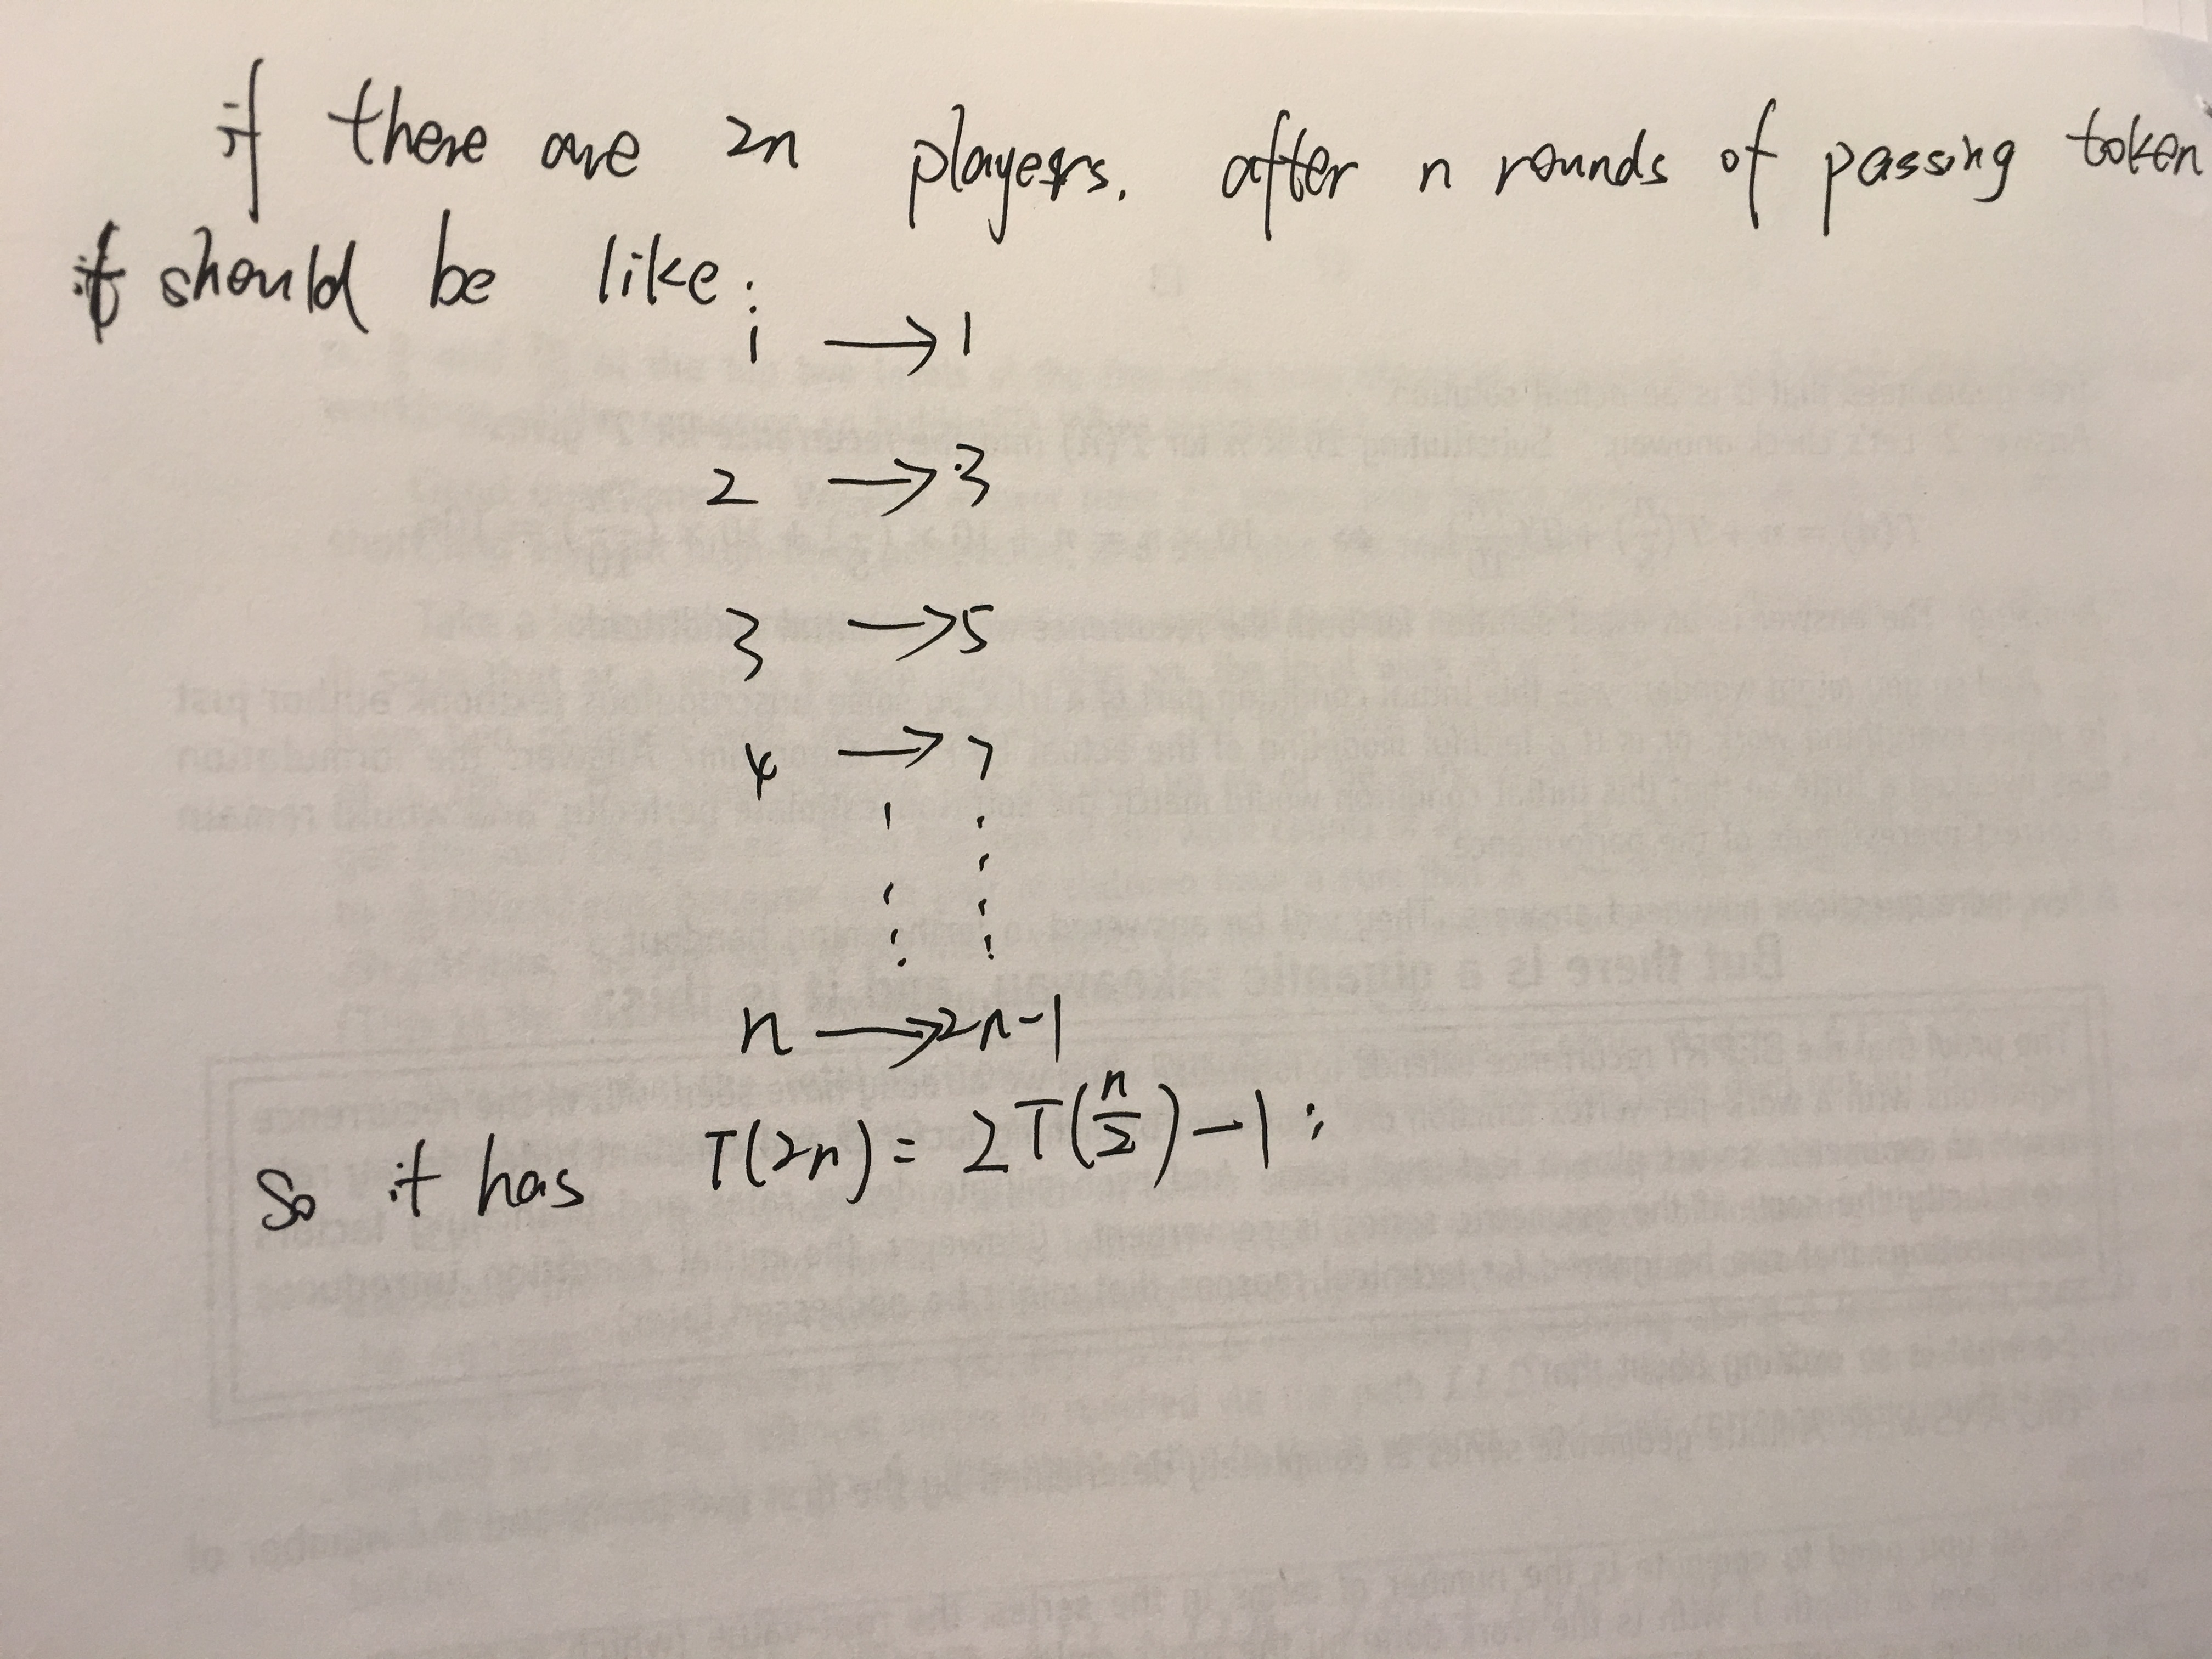
\includegraphics[width=\linewidth]{EX17.jpeg}
  \caption{Exe 3.17 Solution.}
  \label{fig:solution 3.17}
\end{figure}

\begin{math}
  \left\{
    \begin{array}{l}
      $T(1) = 1$             \qquad             if \: n \:  = \: 1;\\
      $T(n) = 2T(n/2) - 1$     \qquad      if  \: n  \: is \: even;\\
      $T(n) = 2T((n-1)/2) + 1$    \quad   if  \: n \:  is \: odd;
    \end{array}
  \right.
\end{math}


\section{Ex 3.18}

\subsection{}
The special value should separate the equation , so it has $T(n) = 1024n + 2T(n/2)$ and $T(n/2) = 4(n/2)^2$  and  $T(n) = 4n^2$.
\begin{equation}
1024n + 4(n/2)^2 = 4n^2
\end{equation}
Hence, $n = 512$.


\subsection{}
\begin{figure}[h!]
  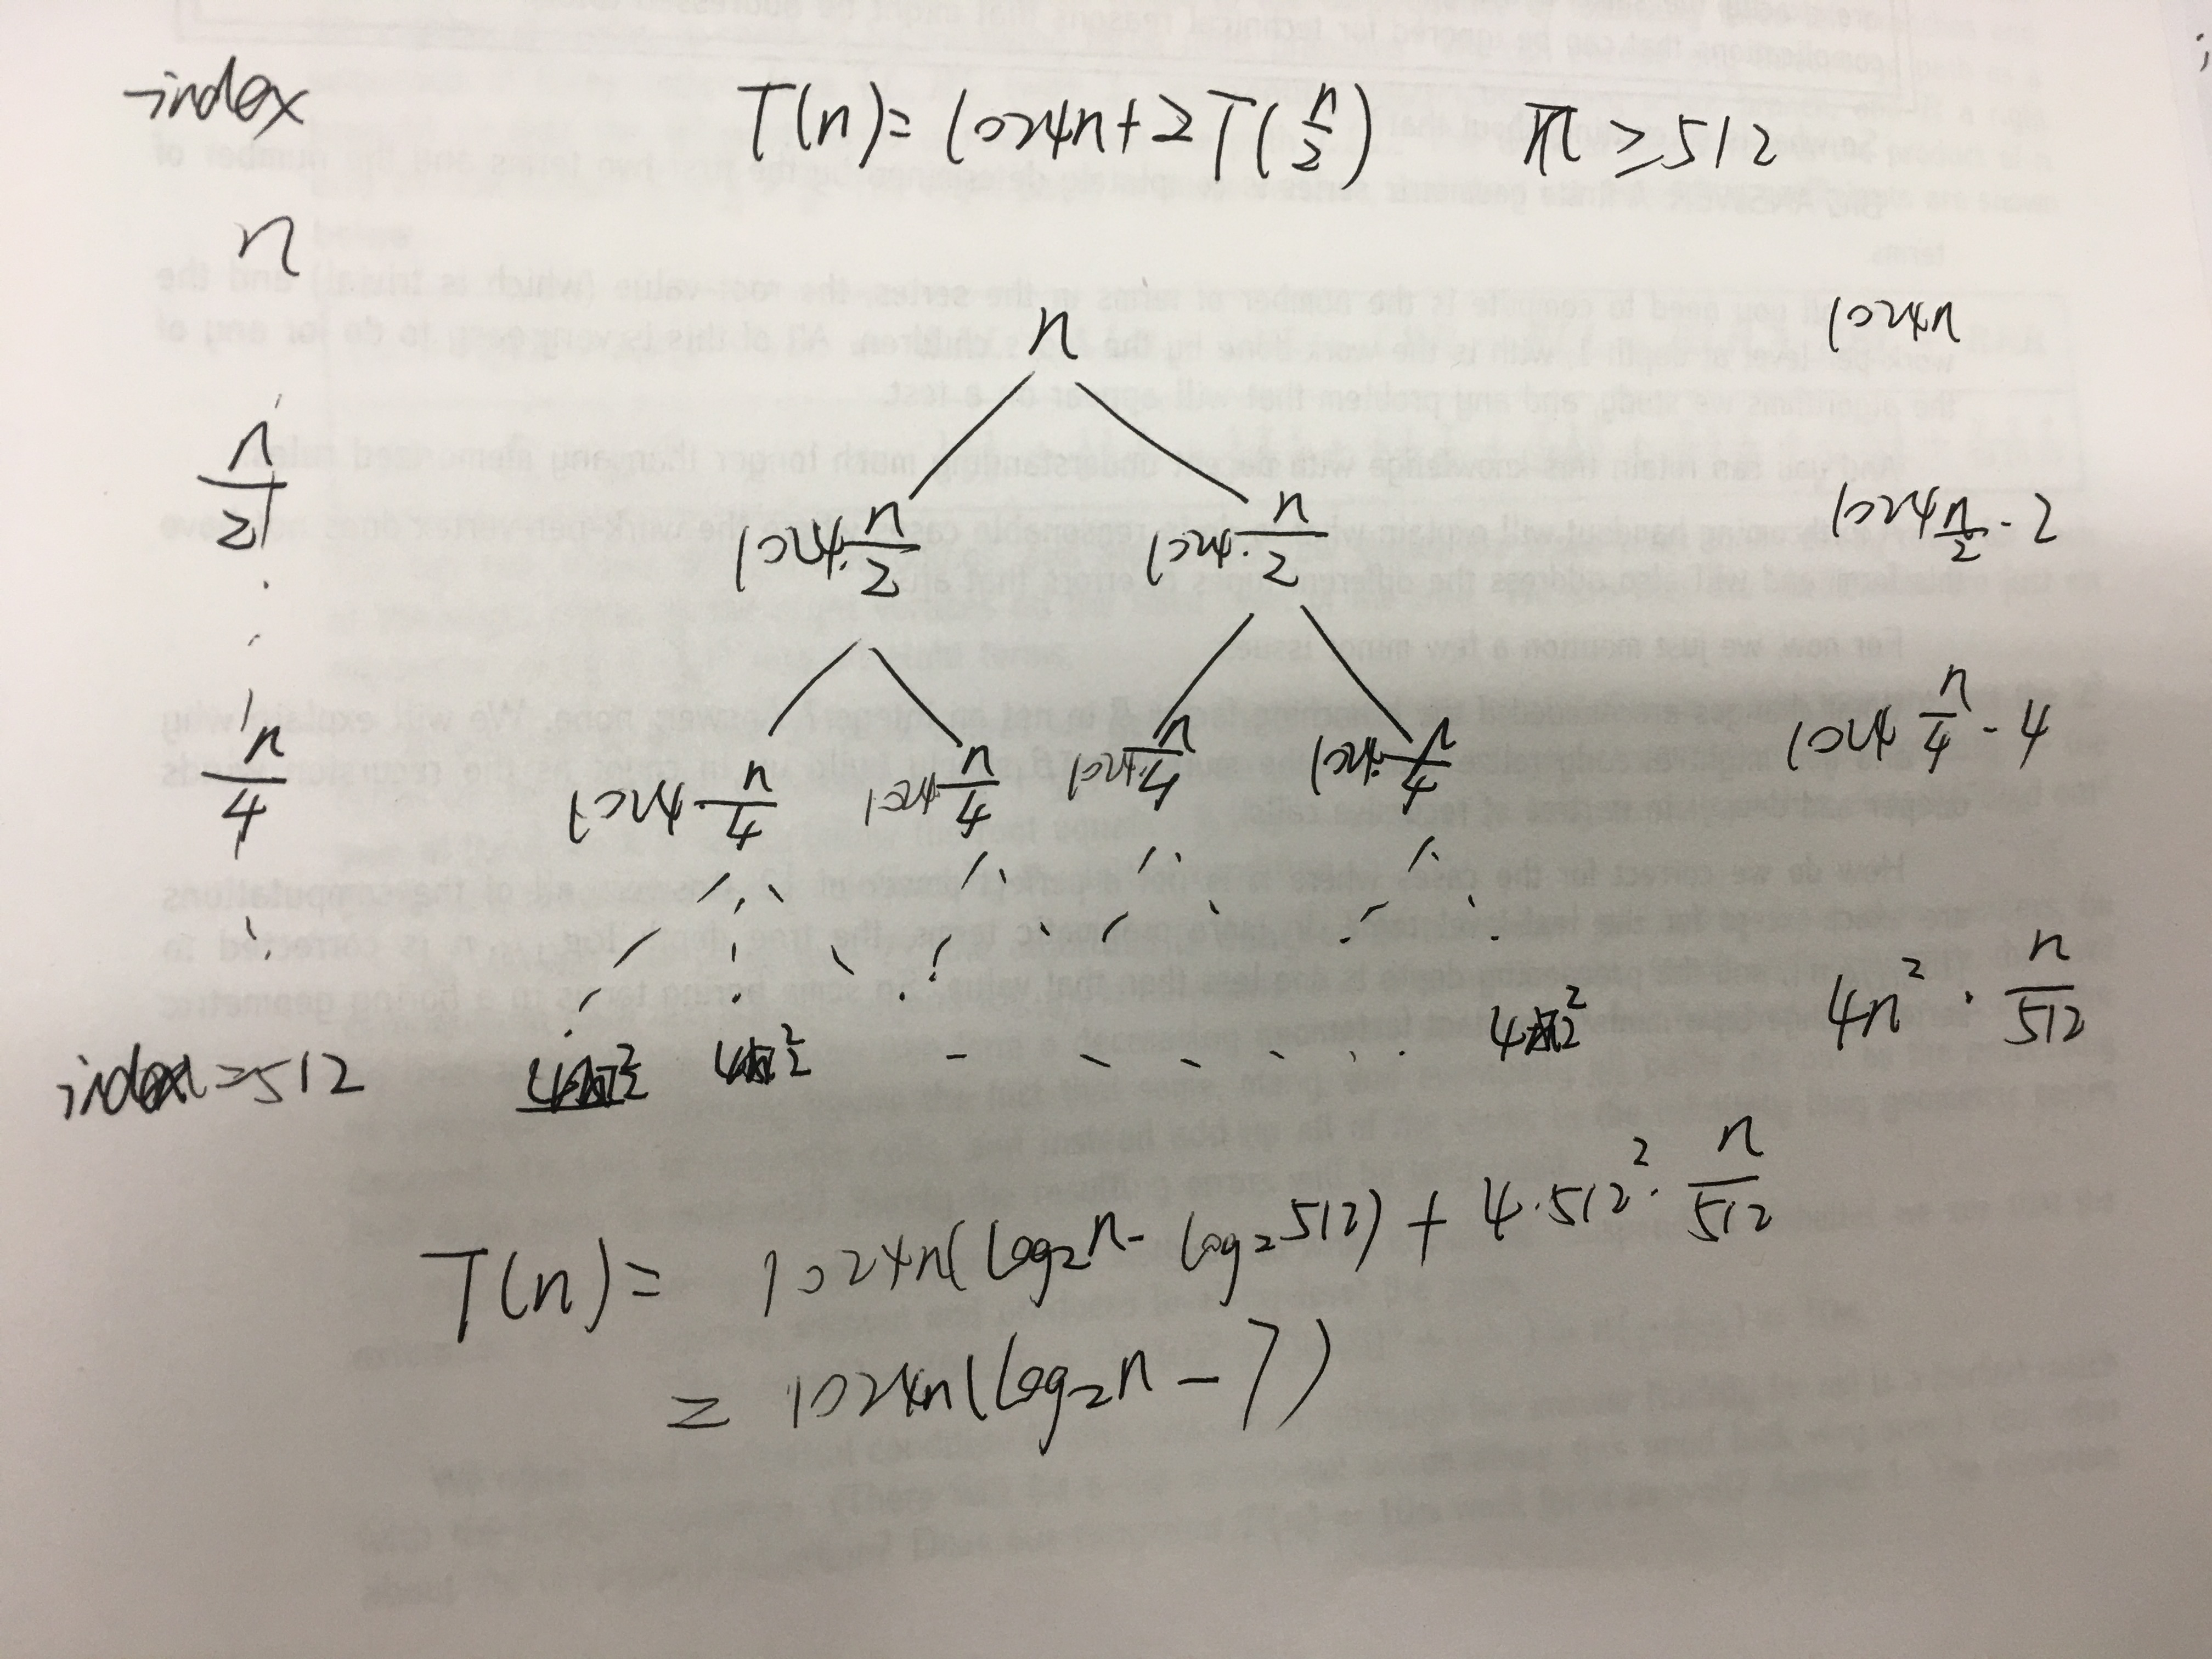
\includegraphics[width=\linewidth]{EX18.jpeg}
  \caption{Exe 3.18 Solution.}
  \label{fig:solution 3.18}
\end{figure}
So \quad $ T(n) = 1024n({\log_2 n} -7)$.


\section{Ex 3.19}
\subsection{}
\begin{math}
  \left\{
    \begin{array}{l}
      $L(0) = 2$             \qquad             if \: k \:  = \: 0;\\
      $L(k) = 2 + 2L(k-1)$     \qquad      if  \: k  \: > \: 0;\\
    \end{array}
  \right.
\end{math}

\subsection{}
\begin{math}
  \left\{
    \begin{array}{l}
      $N(0) = 1$             \qquad             if \: k \:  = \: 0;\\
      $N(k) = 3 + 4N(k-1)$     \qquad      if  \: k  \: > \: 0;\\
    \end{array}
  \right.
\end{math}


\subsection{}
 
$L(k) = 2^{k}+2$     \qquad      if  \: k  \: > \: 0;\\
$N(k) = 3+4^{k}$    \qquad      if  \: k  \: > \: 0;\\
$S(k) = N(k)+1+2L(k)$


\section{Ex 3.28}
\subsection{}
$A(n) = n{\log_2 n}+n$


\subsection{}
$B(n) = n{\log_3 n}+n$

\subsection{}
$C(n) = n^2{\log_2 n}+n^2$

\subsection{}
$D(n) = n^2{\log_3 n}+n^2$ 

\subsection{}
\begin{figure}[H]
  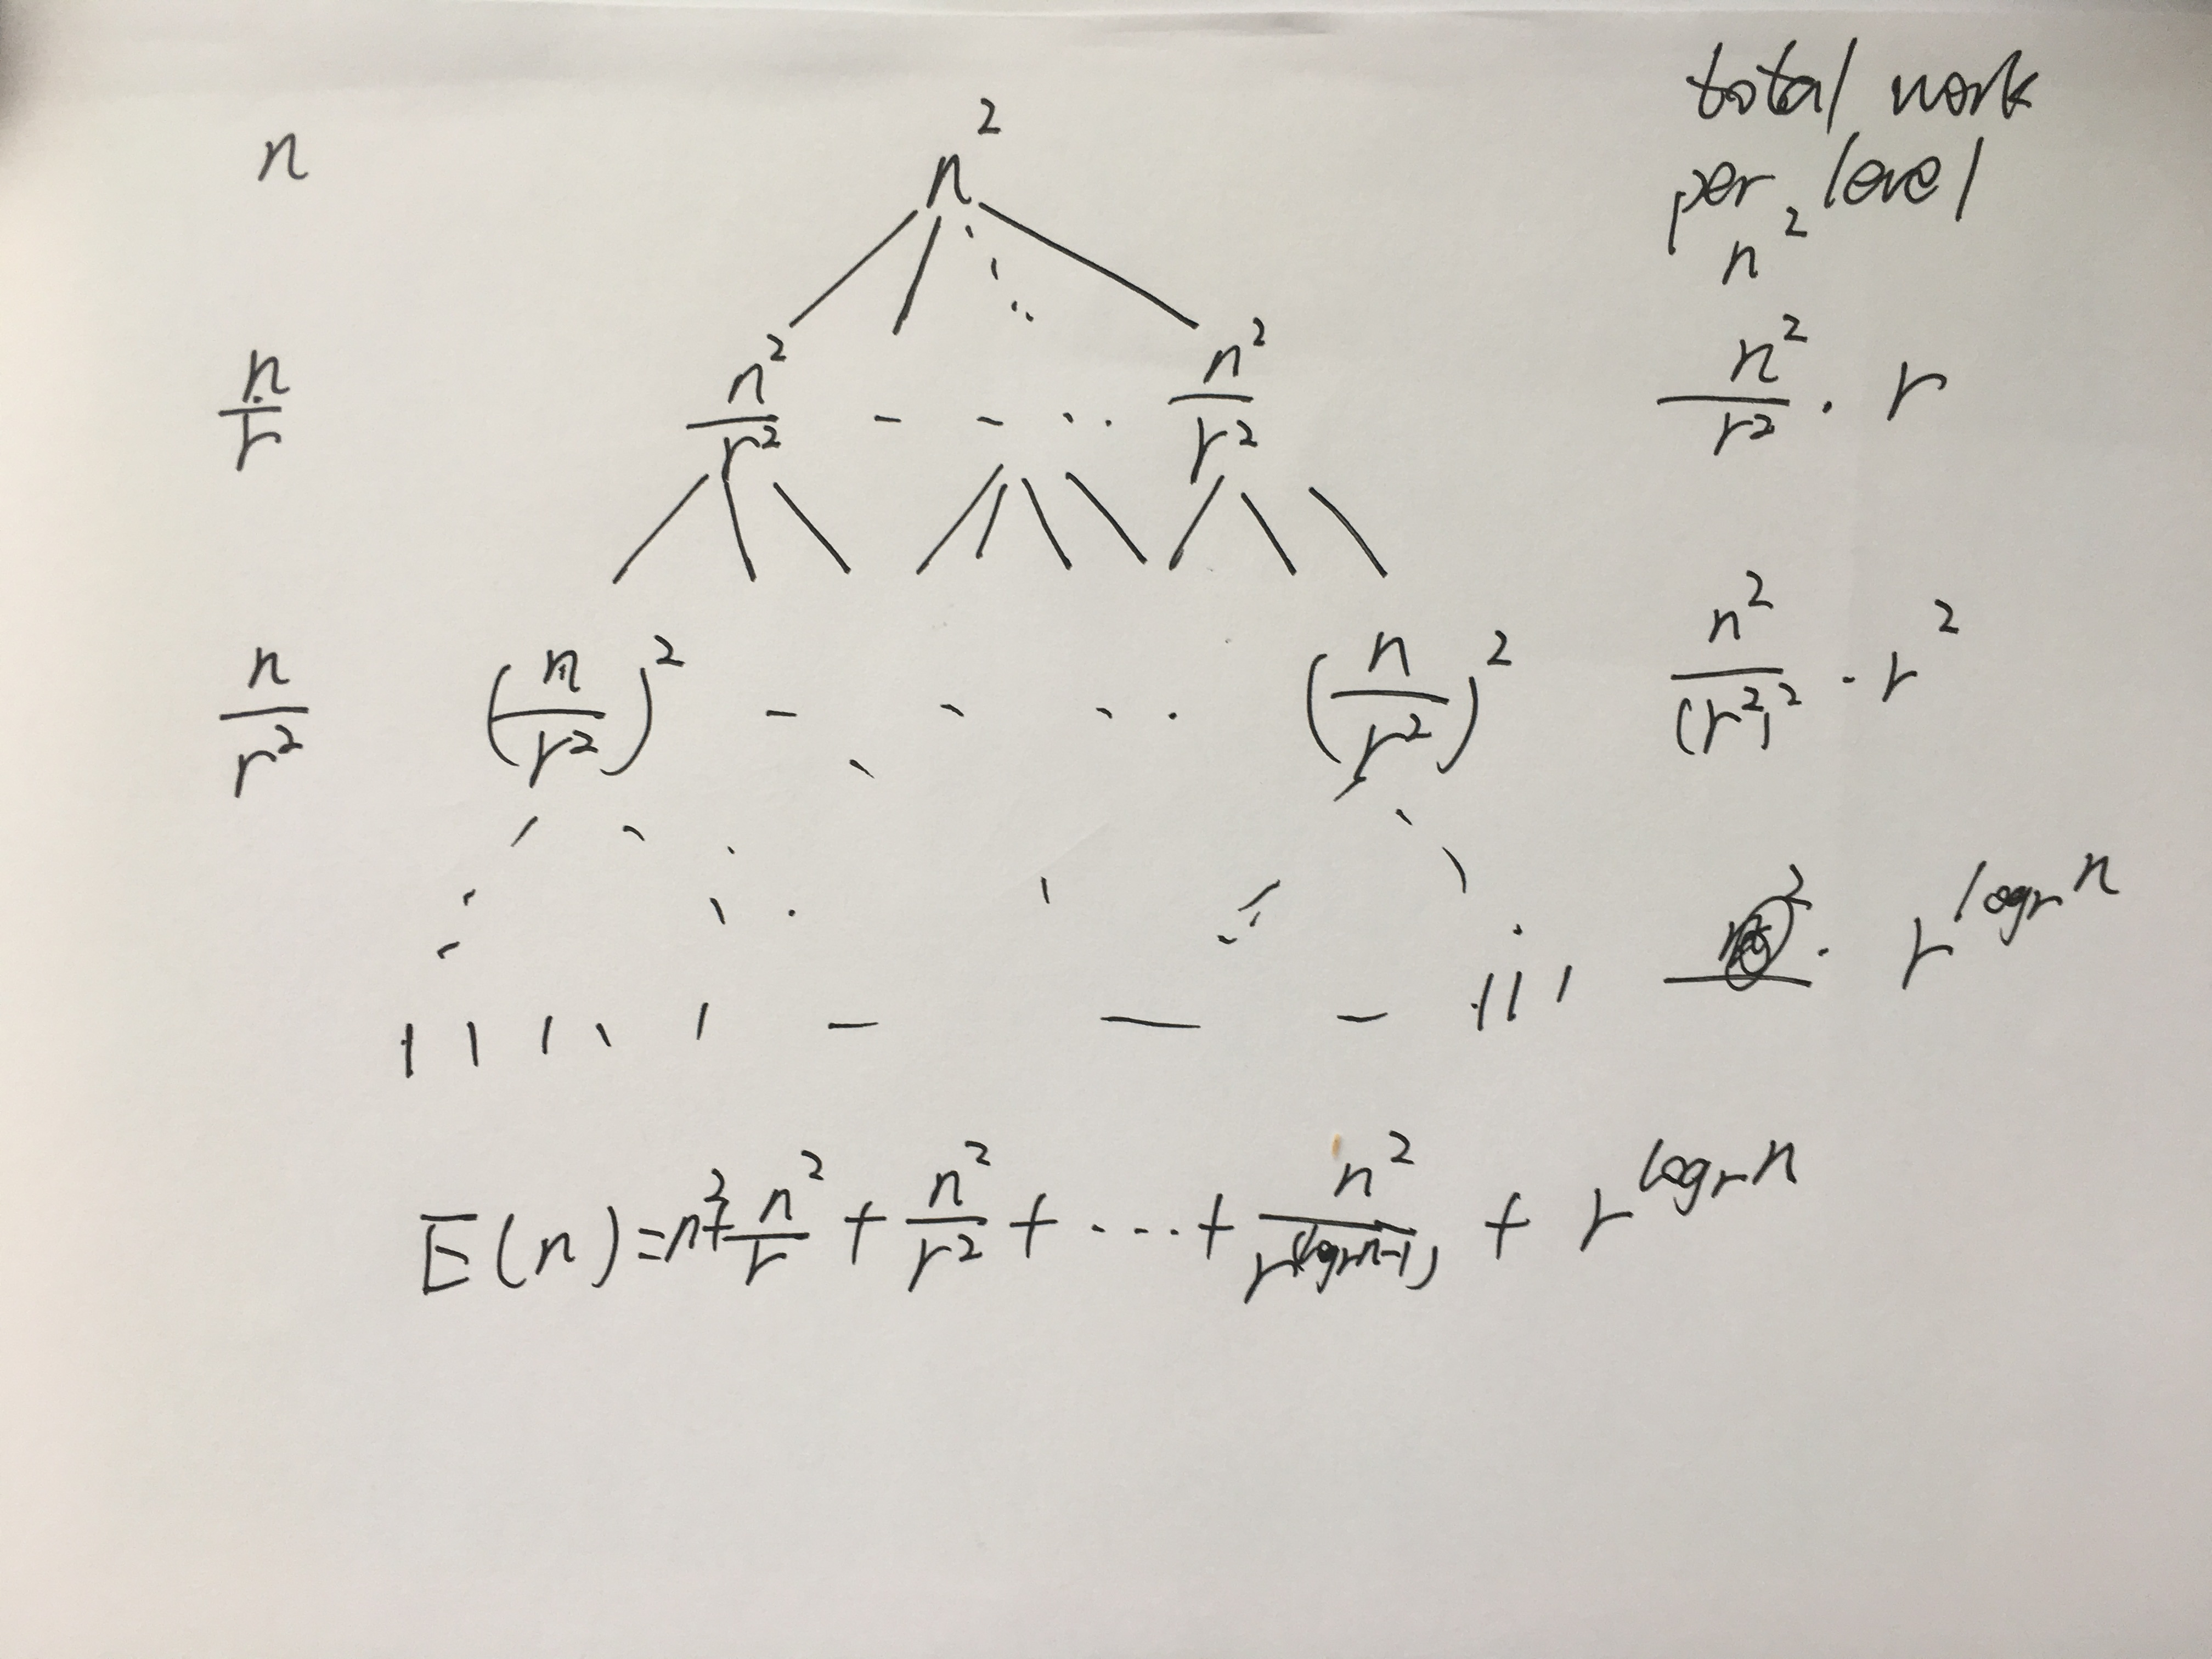
\includegraphics[width=\linewidth]{EX28e.jpeg}
  \caption{Exe 3.28e Solution.}
  \label{fig:solution 3.28e}
\end{figure}

\subsection{}
\begin{figure}[H]
  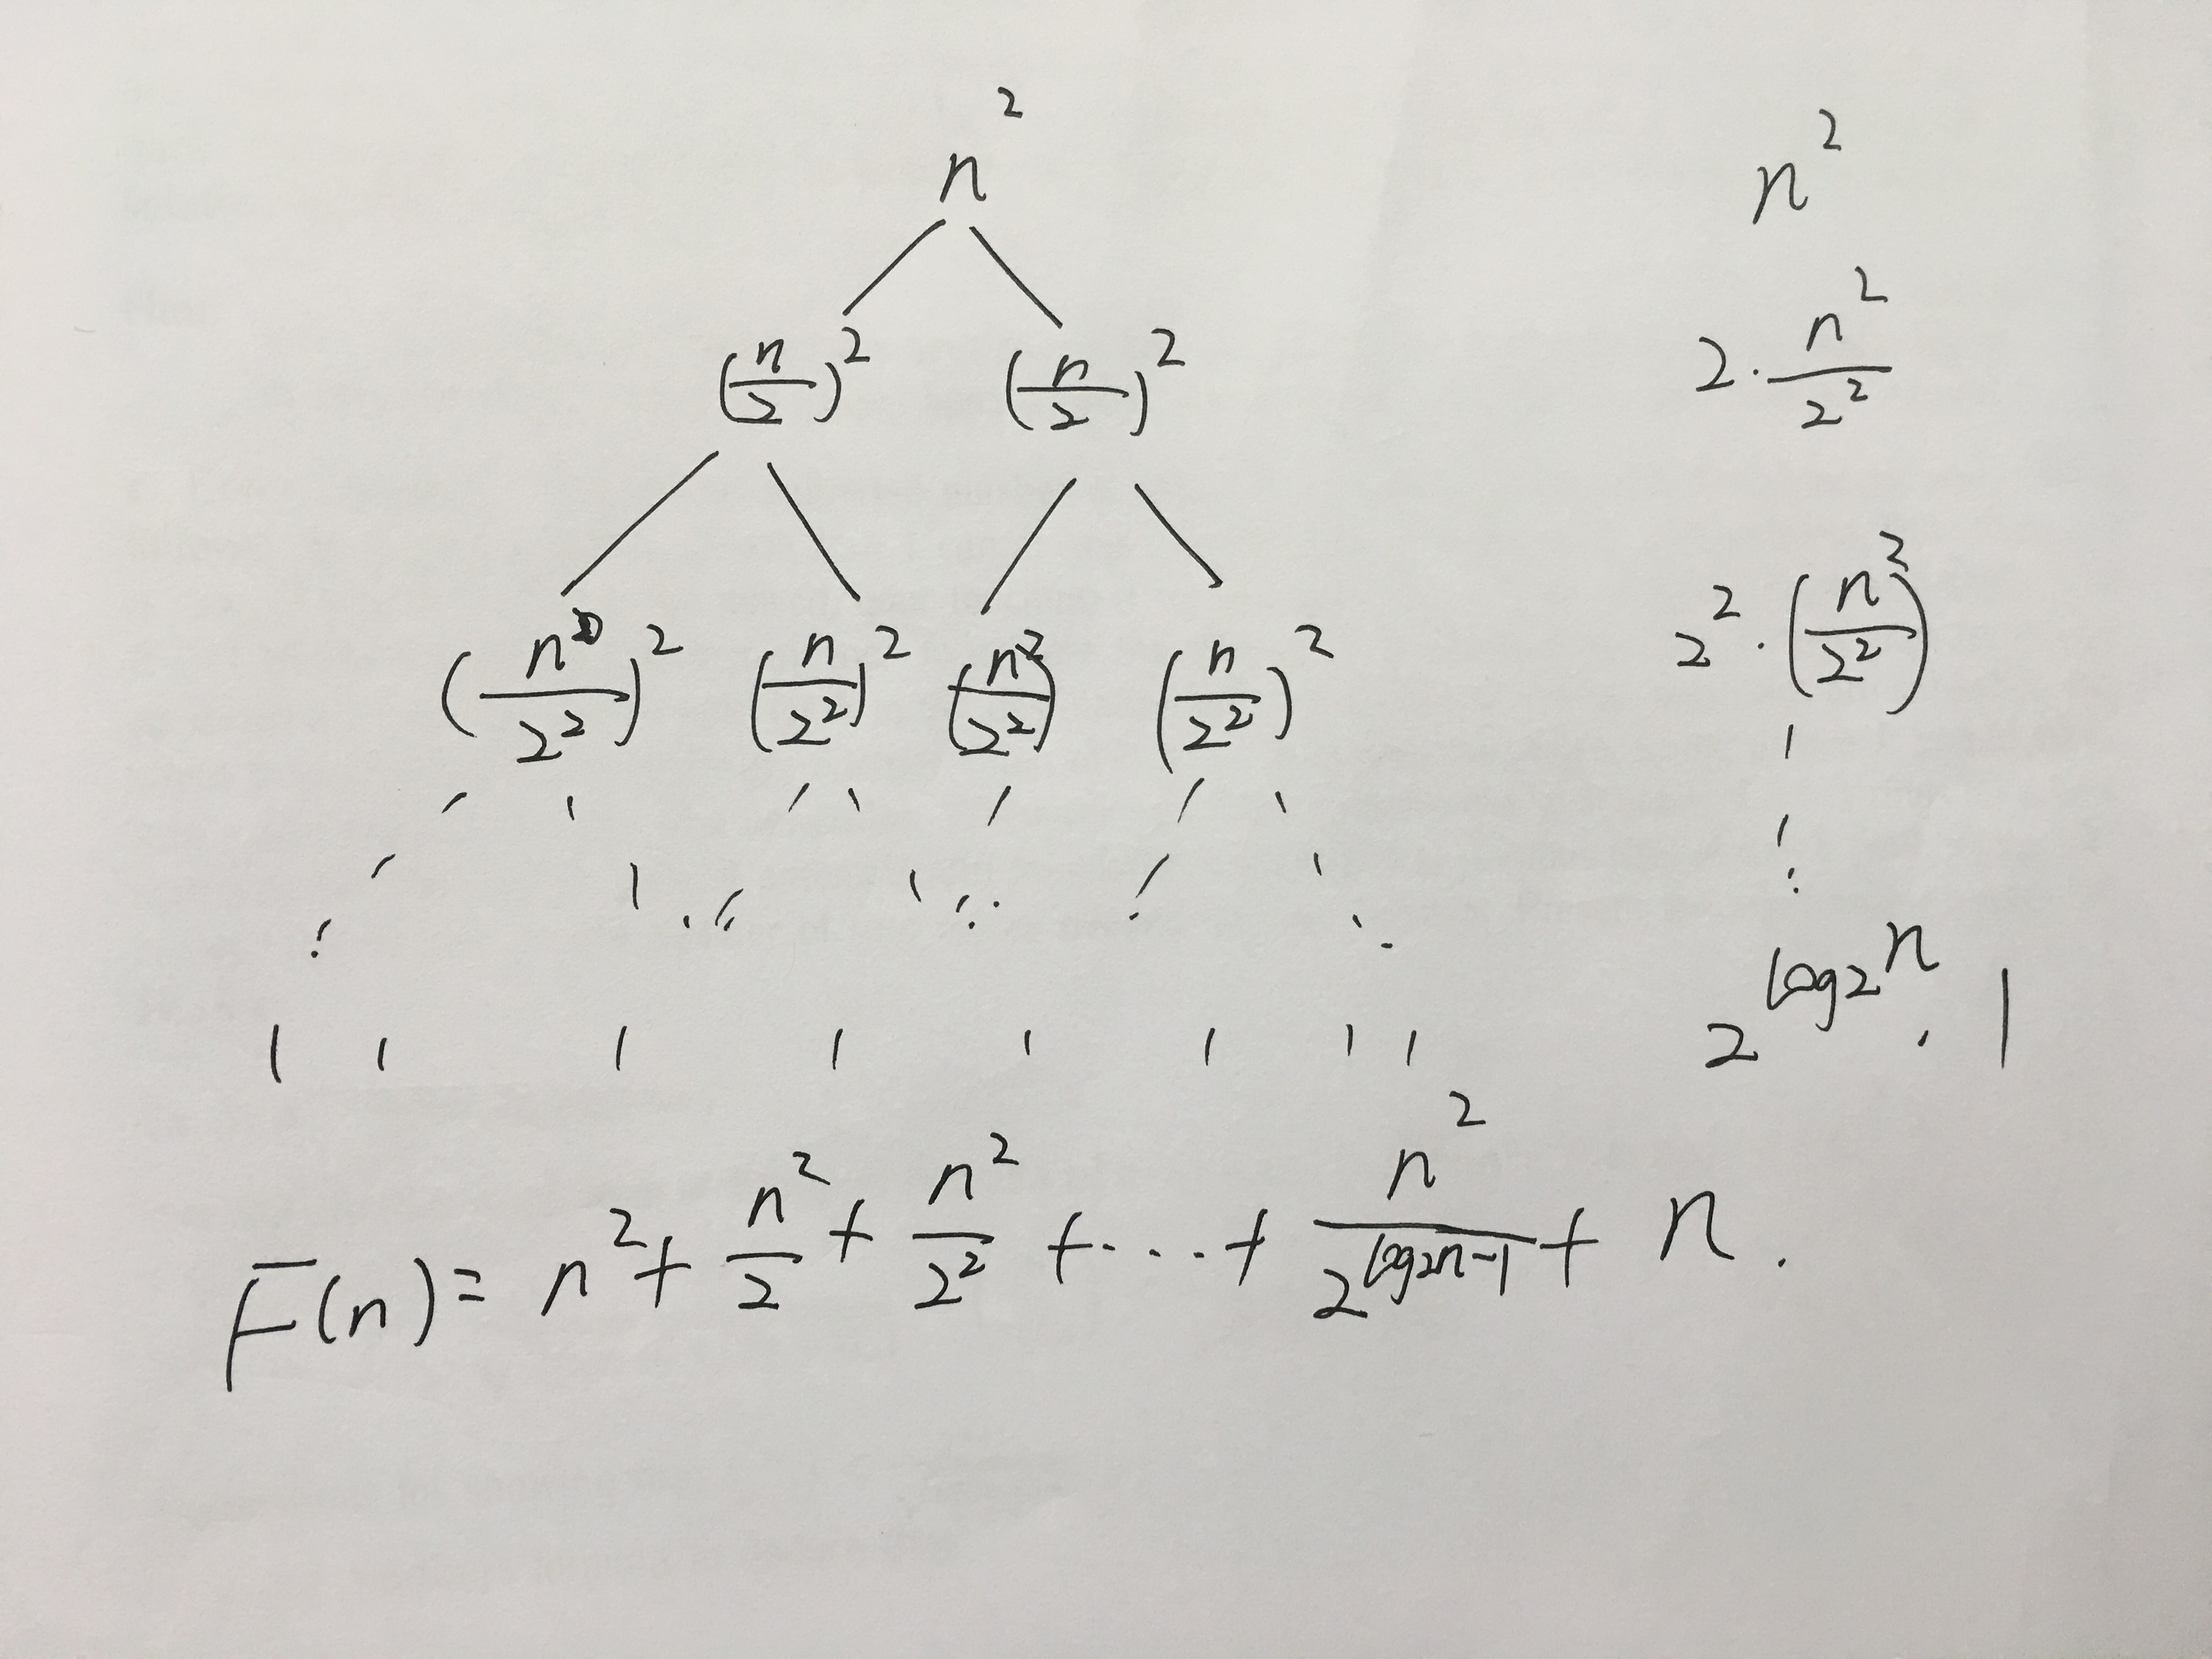
\includegraphics[width=\linewidth]{EX28f.jpeg}
  \caption{Exe 3.28f Solution.}
  \label{fig:solution 3.28f}
\end{figure}

\subsection{}
\subsection{}
\begin{figure}[H]
  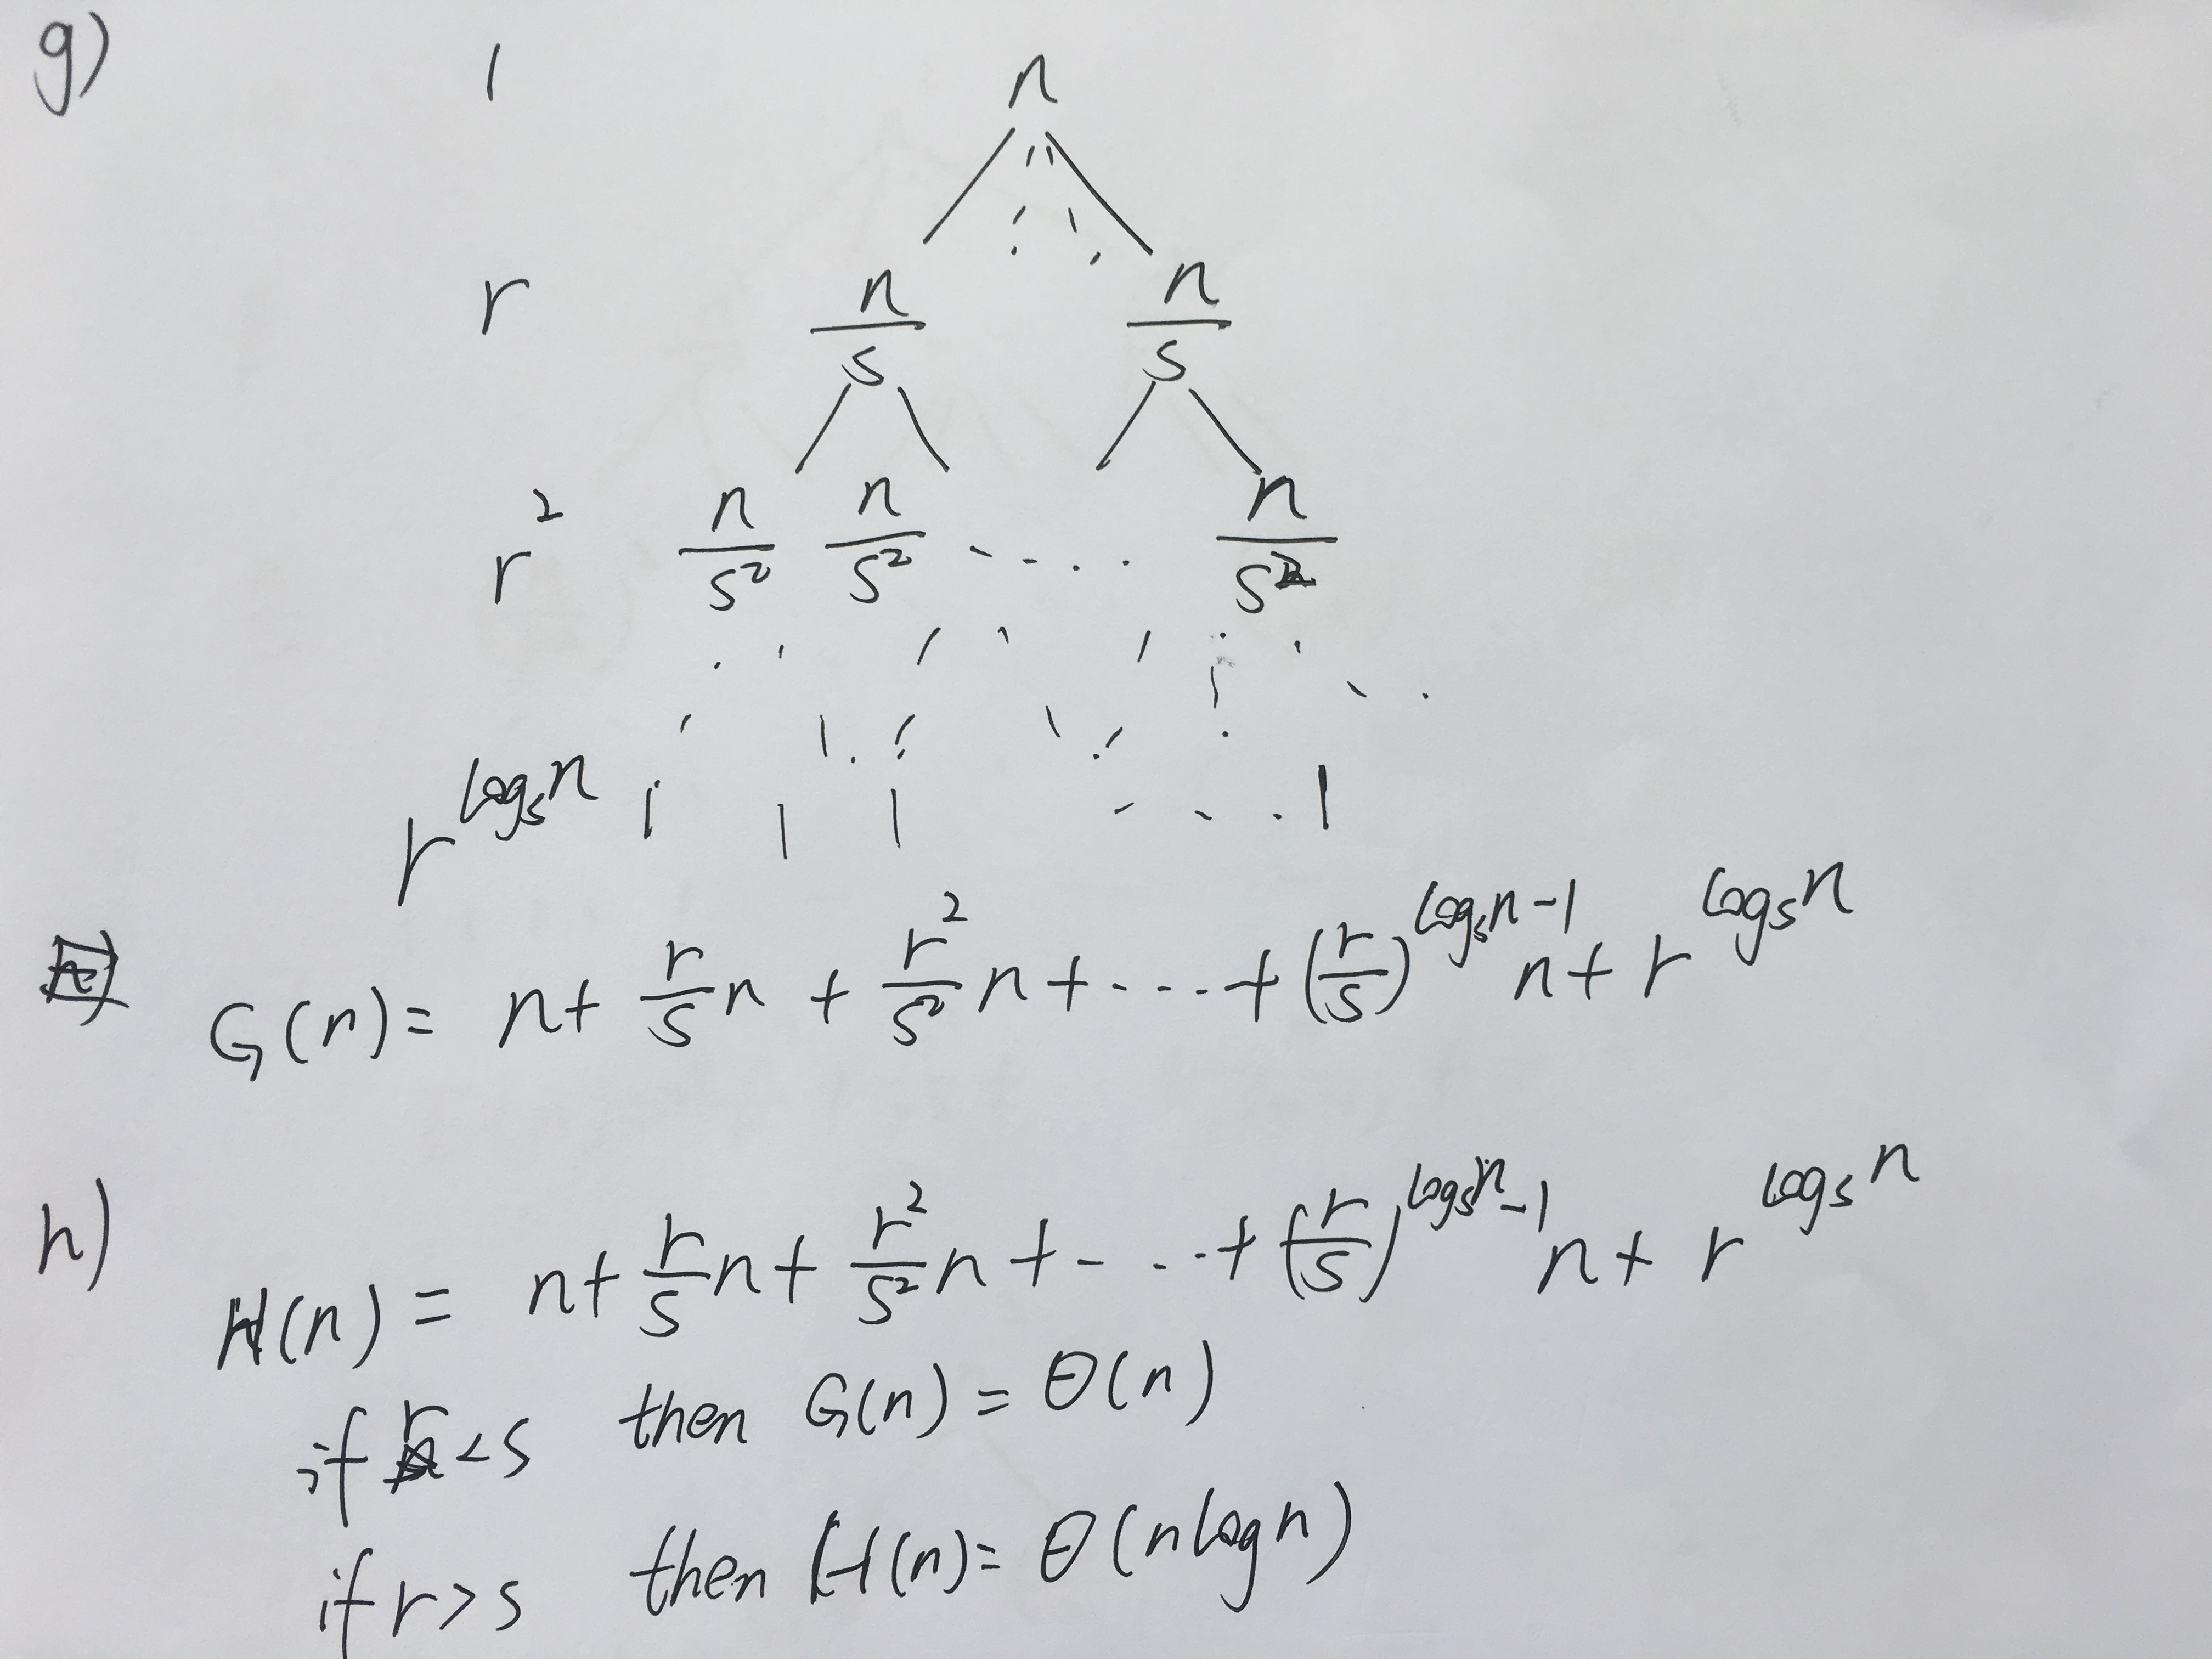
\includegraphics[width=\linewidth]{EX28gh.jpeg}
  \caption{Exe 3.28gh Solution.}
  \label{fig:solution 3.28gh}
\end{figure}

\subsection{}
\subsection{}
\begin{figure}[H]
  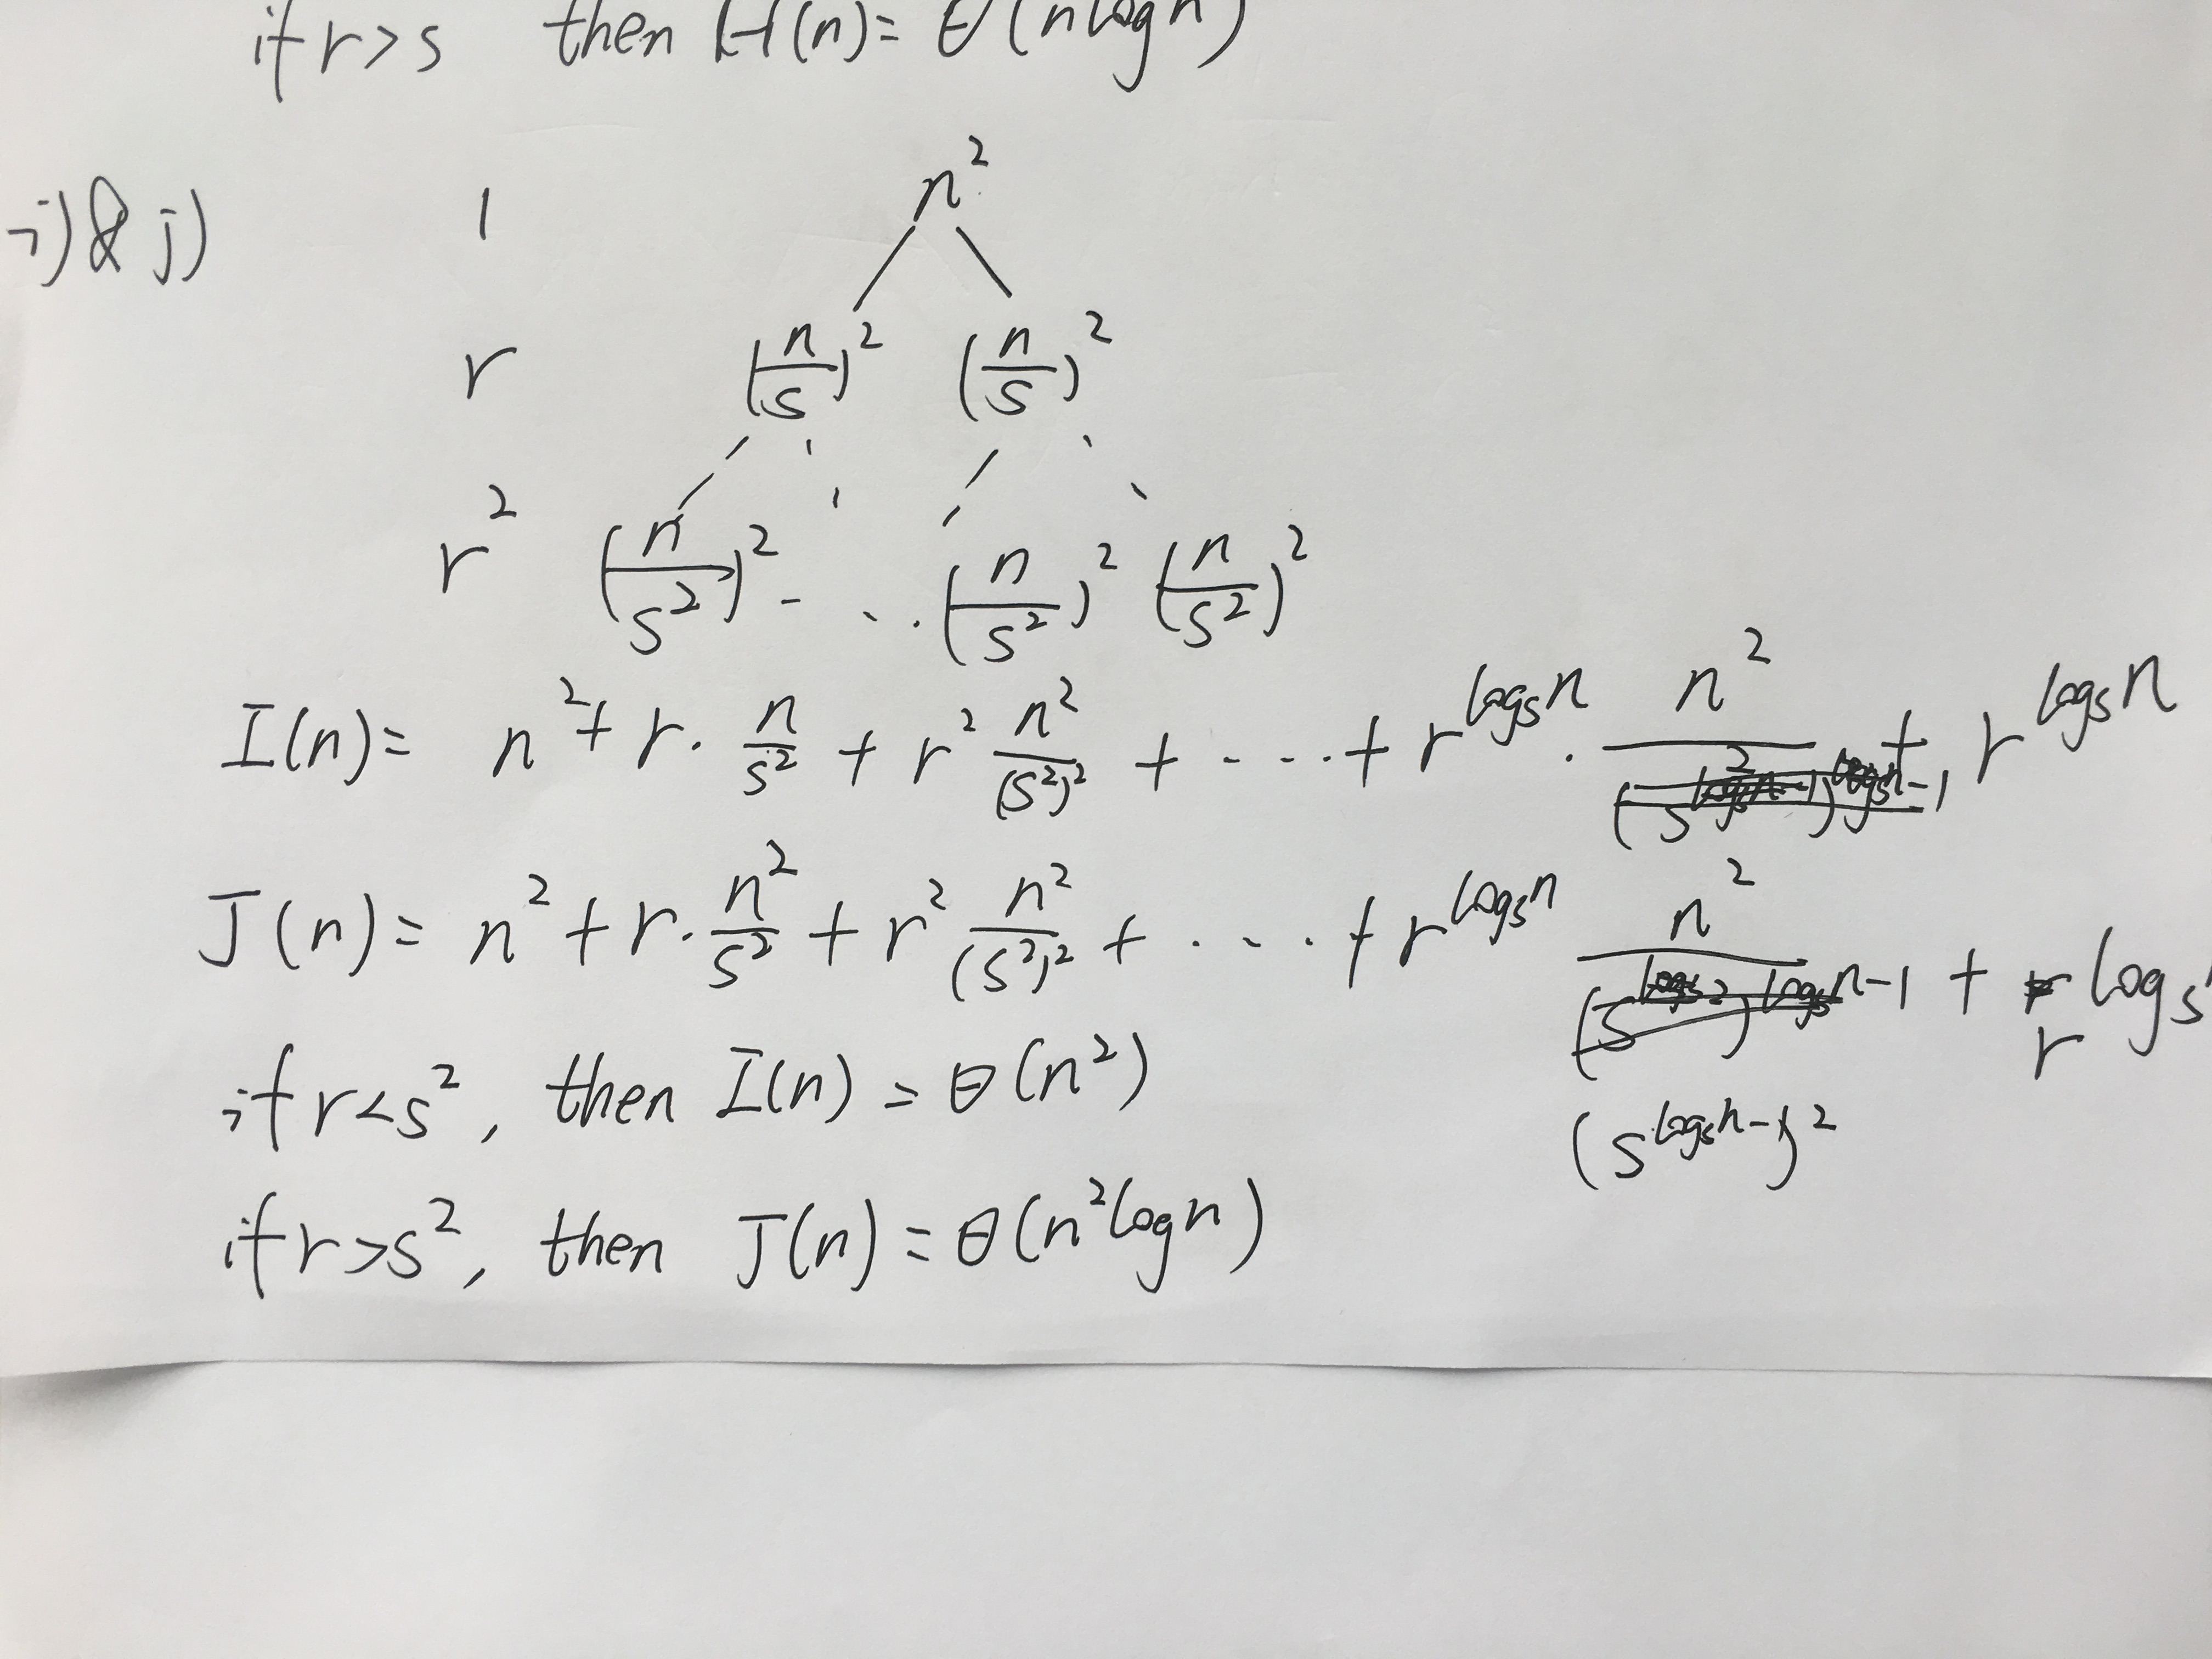
\includegraphics[width=\linewidth]{EX28ij.jpeg}
  \caption{Exe 3.28ij Solution.}
  \label{fig:solution 3.28ij}
\end{figure}

\subsection{}
$K(n) = n^2({\log_3 n}-4) + 81*9^{{(\log_3 n} - 4}$

\subsection{}
$L(n) = {\log_9 n}\sqrt{n} +\sqrt{n} $

\section{3.general}
\begin{figure}[H]
  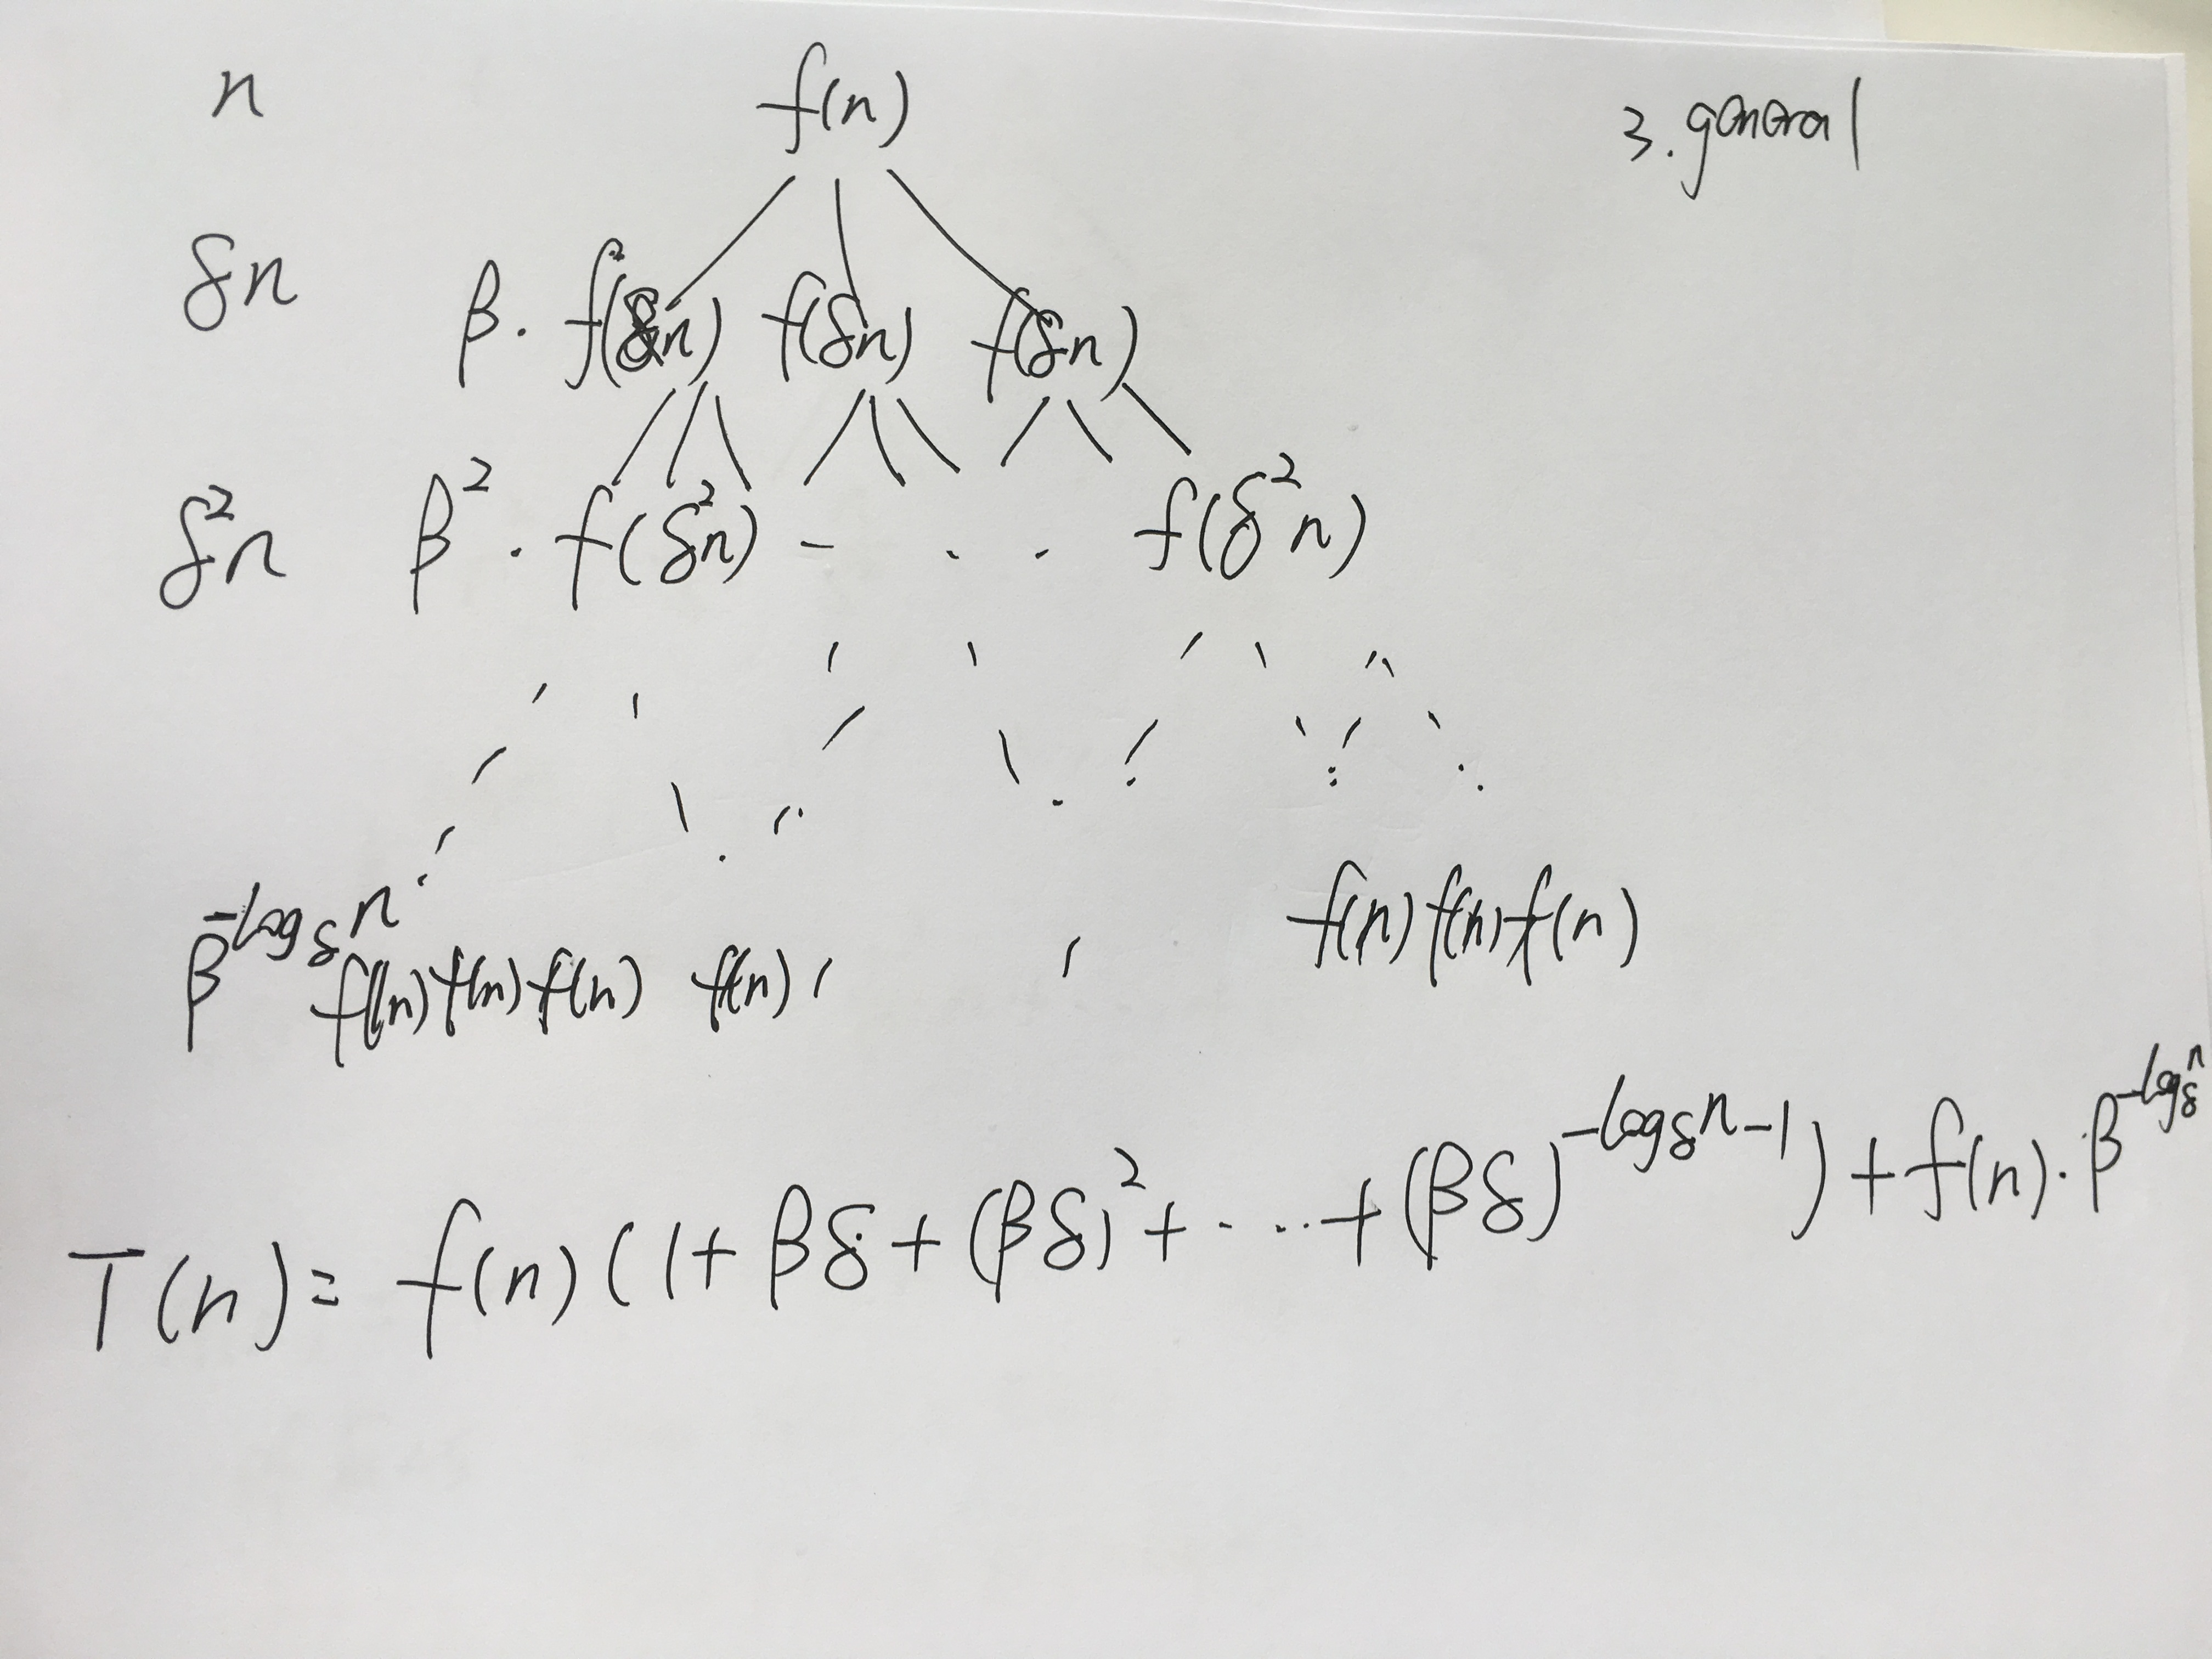
\includegraphics[width=\linewidth]{EXgeneral.jpeg}
  \caption{Exe 3.general Solution.}
  \label{fig:solution 3.general}
\end{figure}

























 
 
 
 
 
 
 
 
 
 
 
 
 
 
 



\end{document}
